% =====================================================================
% RAP-FedWMMSE — IEEE conference paper (Group 12, IIIT Dharwad)
% Template: IEEE Conference Template (IEEEtran), as shared by Sir.
% Revision 1: addresses Google Deep Review round 1 (see REVISION_LOG.md).
%
% Note: teammate emails use the institute pattern <rollno>@iiitdwd.ac.in —
% verify them before submission.
% Every number in this paper comes from the saved final results
% (rapfedbeam/results/*.json, 100 drops over 10 deployments) or the
% committed figure CSVs in rapfedbeam/figures/.
% =====================================================================
\documentclass[conference]{IEEEtran}
\IEEEoverridecommandlockouts

\usepackage{cite}
\usepackage{amsmath,amssymb,amsfonts}
\usepackage{graphicx}
\usepackage{booktabs}
\usepackage{algorithm}
\usepackage{algpseudocode}
\usepackage{textcomp}
\usepackage{xcolor}
\usepackage{url}

\graphicspath{{figures/}}

\makeatletter
\newcommand{\linebreakand}{%
  \end{@IEEEauthorhalign}\hfill\mbox{}\par
  \mbox{}\hfill\begin{@IEEEauthorhalign}}
\makeatother

\newcommand{\norm}[1]{\left\lVert #1 \right\rVert}
\newcommand{\abs}[1]{\left\lvert #1 \right\rvert}
\newcommand{\herm}{^{\mathsf{H}}}
\newcommand{\C}{\mathbb{C}}
\newcommand{\R}{\mathbb{R}}
\newcommand{\sgn}{\operatorname{sg}}
\newcommand{\zs}{\boldsymbol{\zeta}_{\mathrm{s}}}
\newcommand{\zf}{\boldsymbol{\zeta}_{\mathrm{f}}}
\newcommand{\Loss}{\mathcal{L}}

\begin{document}

\title{RAP-FedWMMSE: Role-Aware Personalized Federated Beam Optimization for
Intelligent-Relay-Assisted Cell-Free Massive MIMO\\
}

\author{
\IEEEauthorblockN{Kushagra Kumar Arora}
\IEEEauthorblockA{\textit{Indian Institute of Information}\\
\textit{Technology Dharwad} (24BCS061)\\
Dharwad, India \\
24bcs061@iiitdwd.ac.in}
\and
\IEEEauthorblockN{Chinmay Pramod Ardalkar}
\IEEEauthorblockA{\textit{Indian Institute of Information}\\
\textit{Technology Dharwad} (24BEC007)\\
Dharwad, India \\
ardalkarchinmay10@gmail.com}
\linebreakand
\IEEEauthorblockN{Rachit Yadav}
\IEEEauthorblockA{\textit{Indian Institute of Information}\\
\textit{Technology Dharwad} (24BEC049)\\
Dharwad, India \\
24bec049@iiitdwd.ac.in}
\and
\IEEEauthorblockN{Saurav Anand Jha}
\IEEEauthorblockA{\textit{Indian Institute of Information}\\
\textit{Technology Dharwad} (24BEC054)\\
Dharwad, India \\
24bec054@iiitdwd.ac.in}
}

\maketitle

\begin{abstract}
Cell-free massive MIMO serves every user from many distributed access points
(APs), but blocked users still see weak direct links, and centralized beam
optimization requires full channel state information (CSI) at a central
processor. We study \emph{RAP-FedWMMSE}, a model-driven algorithm in which
APs and half-duplex decode-and-forward relays optimize their beams from local
CSI plus exchanged coordination quantities. It combines slow-timescale relay
association and phase-split adaptation with fast-timescale unfolded
per-node weighted-MMSE (WMMSE) layers whose step sizes, relaxation and
regularization are predicted by role-specific neural models trained
self-supervised on the network utility, with no dataset. Primal--dual prices
handle quality-of-service and decode-and-forward bottlenecks, and an
event-triggered, compressed, personalized federated exchange shares model
updates under fronthaul limits. Over 14 experiments of 100 user drops on 10
deployments, with a certified global bound from spatial branch-and-bound on a
small network, RAP-FedWMMSE reaches 76\% of the centralized benchmark's mean
rate and gains $+11.3$ proportional-fair (PF) utility over uncoordinated
Local-WMMSE. A paired decomposition attributes $+7.3$ of this to the
coordination exchanged between nodes, $+3.1$ to slow-timescale phase-split and
association adaptation, and only $+0.9$ to the learned layer parameters. The
method overtakes the centralized relay-assisted benchmark under stale CSI and
saves 22\% power for a 0.14 utility loss. Federated aggregation brings no
measurable utility gain over local training in our setting; its benefit is
45\% less communication than FedAvg.
\end{abstract}

\begin{IEEEkeywords}
cell-free massive MIMO, relays, WMMSE, deep unfolding, federated learning,
beamforming, resource allocation
\end{IEEEkeywords}

\section{Introduction}
Cell-free massive MIMO replaces cells with a dense set of access points (APs)
that serve all users jointly~\cite{ngo2017cellfree,interdonato2019ubiquitous}.
Its weakest link is the user whose direct channels to every nearby AP are
blocked: no amount of coherent combining recovers a link that is 25\,dB down.
Half-duplex decode-and-forward (DF) relays~\cite{cover1979relay,%
laneman2004cooperative} can restore such users, at the price of a two-phase
frame, a relay-decoding bottleneck, and a binary association problem coupled
to the beam design.

The resulting joint design --- transmit beams at every AP, forwarding beams
and receive combiners at every relay, the relay--user association, and the
phase split $\tau$ --- is a mixed-integer nonlinear program (MINLP).
Centralized weighted-MMSE (WMMSE) methods~\cite{shi2011wmmse,%
christensen2008wmmse} solve the continuous part well but require all
instantaneous CSI at a central processor. Deep
unfolding~\cite{monga2021unrolling,chowdhury2021unfolding} keeps the structure
of a proven optimizer and learns only a few interpretable parameters.

This paper implements and evaluates \emph{RAP-FedWMMSE} (role-aware
personalized federated WMMSE), a model-driven distributed algorithm with the
following components:
\begin{itemize}
  \item \textbf{Relay association} by a capacitated matching on large-scale
    gains, solved exactly as a binary program, with cooperation order
    $L_{\max}\ge1$.
  \item \textbf{Unfolded per-node WMMSE layers}: every AP and relay runs $L$
    layers of a regularized WMMSE step whose step size, relaxation and
    regularization are predicted from local CSI and a slow coordination vector
    by a role-specific adapter, a personalized backbone and a head. With
    neutral parameters a layer is exactly the classical per-node WMMSE update.
  \item \textbf{Primal--dual corrections} for the QoS target and the DF
    bottleneck, and a robust loss with a CSI-error outage surrogate.
  \item \textbf{Self-supervised training with no dataset}: the loss is the
    network utility itself, evaluated on simulated channels.
  \item \textbf{Personalized federated learning} with event triggering, exact
    knapsack client selection under per-node fronthaul headroom, top-$k$
    compression with error feedback, and topology- and role-aware
    aggregation.
\end{itemize}

The evaluation compares fair baselines (the no-relay benchmark uses the whole
frame, $\tau=1$), a certified MINLP bound on a small network, and paired
statistics over the same 100 drops. Besides the overall ranking, we decompose
where the proposed method's gain comes from, and we report the results that
did not support our hypotheses.

\section{Related Work}
\textbf{WMMSE and its descendants.} WMMSE~\cite{shi2011wmmse} converts
weighted sum-rate maximization into an alternating minimization over
receivers, MSE weights and beams; the rate--MSE relationship originates
in~\cite{christensen2008wmmse}. Our centralized benchmark extends it to a
two-phase DF rate with a log utility via successive convex approximation
(SCA), keeping the DF $\min$ and the logarithm exact.

\textbf{Deep unfolding of WMMSE.} Algorithm unrolling~\cite{monga2021unrolling}
learns the internal parameters of an iterative algorithm.
\cite{chowdhury2021unfolding} unfolds WMMSE with graph neural networks for
power allocation. Unfolded WMMSE has been extended to multiuser MIMO
precoding~\cite{hu2021iaidnn}, made matrix-inverse-free for parallel
hardware~\cite{pellaco2022inversefree}, and distributed over multicell
MU-MIMO networks with local CSI and graph-based coordination between base
stations~\cite{schynol2023gcnwmmse}. RAP-FedWMMSE follows this line; what it
adds is the two-phase half-duplex DF relay structure, AP/relay role-specific
models, primal--dual QoS/DF pricing inside the layers, and federated training
of the models under fronthaul limits.

\textbf{Distributed and relay-assisted cell-free MIMO.} Team MMSE
precoding~\cite{miretti2022team} gives optimal distributed precoding for
cell-free networks with local CSI. Relay-type assistance has been analyzed for
cell-free systems with hybrid relay--reflecting surfaces~\cite{nguyen2023hrris}
and with multipair DF relaying under network-assisted full
duplex~\cite{vu2023dfrelay}. We consider half-duplex DF relays with joint
optimization of beams, combiners, association and phase split.

\textbf{Federated learning.} FedAvg~\cite{mcmahan2017fedavg} averages client
updates; personalized FL~\cite{tan2022personalized} adapts models to
heterogeneous clients; sparse uploads with error feedback follow
\cite{aji2017sparse}. Federated learning has been applied to precoding design
in cell-free massive MIMO~\cite{wang2023flprecoding}. Here FL shares the
parameters of the models that drive the unfolded layers, and the fronthaul
constraint of the network limits the FL traffic itself.

\textbf{Exact benchmarks.} Spatial branch-and-bound in
SCIP~\cite{bestuzheva2021scip} certifies global bounds for small nonconvex
MINLPs; we use it to measure true optimality gaps.

\section{System Model}
\subsection{Network and frame structure}
$M$ APs with $N_A$ antennas, $R$ half-duplex DF relays with $N_R$ antennas and
$K$ single-antenna users (UEs) share one coherence block of unit length, split
into two phases. In Phase~I, of duration $\tau$, the APs transmit; UEs and
relays listen. In Phase~II, of duration $1-\tau$, the relays forward the
streams of their assisted UEs; the APs are silent. Each UE $k$ is served by a
cluster of its $L_c$ strongest APs, encoded by $c_{mk}\in\{0,1\}$, and may be
assisted by relays through the binary association $a_{rk}\in\{0,1\}$ with
$\sum_r a_{rk}\le L_{\max}$ and $\sum_k a_{rk}\le C_r^{\max}$. We write
$\mathbf{W}=\{\mathbf{w}_{mk}\}$, $\mathbf{V}=\{\mathbf{v}_{rk}\}$,
$\mathbf{U}=\{\mathbf{u}_{rk}\}$ and $\mathbf{A}=[a_{rk}]$.

Channels are $\mathbf{h}_{mk}\in\C^{N_A}$ (AP $m$ to UE $k$),
$\mathbf{G}_{mr}\in\C^{N_R\times N_A}$ (AP $m$ to relay $r$) and
$\mathbf{g}_{rk}\in\C^{N_R}$ (relay $r$ to UE $k$), drawn as independent
Rayleigh fading over 3GPP UMi NLOS path loss with log-normal shadowing. A
fraction of UEs is blocked: their direct AP--UE links suffer an extra 25\,dB
loss, while their relay links do not. Channels are normalized by the noise
power, so $\sigma^2=\sigma_r^2=1$ below and beam powers are in Watts.

\subsection{Rates and modeling assumptions}
AP $m$ precodes stream $k$ with $\mathbf{w}_{mk}\in\C^{N_A}$
($\mathbf{w}_{mk}=\mathbf{0}$ unless $c_{mk}=1$); relay $r$ forwards stream
$k$ with $\mathbf{v}_{rk}\in\C^{N_R}$ ($\mathbf{v}_{rk}=\mathbf{0}$ unless
$a_{rk}=1$) and receives it with a unit-norm combiner
$\mathbf{u}_{rk}\in\C^{N_R}$. With receive gains written as
$\mathbf{h}\herm\mathbf{w}$, the Phase~I SINR at UE $k$, the relay-decoding
SINR at relay $r$, and the Phase~II SINR at UE $k$ are
\begin{align}
\gamma_k^{(1)} &= \frac{\abs{\sum_m \mathbf{h}_{mk}\herm \mathbf{w}_{mk}}^2}
 {\sum_{j\ne k}\abs{\sum_m \mathbf{h}_{mk}\herm \mathbf{w}_{mj}}^2 + \sigma^2},
 \label{eq:sinr1}\\
\gamma_{rk}^{AR} &= \frac{\abs{\mathbf{u}_{rk}\herm \mathbf{f}_{rk}}^2}
 {\sum_{j\ne k}\abs{\mathbf{u}_{rk}\herm \mathbf{f}_{rj}}^2 + \sigma_r^2},
 \quad \mathbf{f}_{rj} = \textstyle\sum_m \mathbf{G}_{mr}\mathbf{w}_{mj},
 \label{eq:sinrAR}\\
\gamma_k^{(2)} &= \frac{\abs{\sum_r \mathbf{g}_{rk}\herm \mathbf{v}_{rk}}^2}
 {\sum_{j\ne k}\abs{\sum_r \mathbf{g}_{rk}\herm \mathbf{v}_{rj}}^2 + \sigma^2}.
 \label{eq:sinr2}
\end{align}
The destination capacity, the relay-hop capacity and the DF rate of UE $k$
(in bit/s/Hz) are
\begin{align}
C_k^{D} &= \tau\log_2\!\bigl(1+\gamma_k^{(1)}\bigr)
          + (1-\tau)\log_2\!\bigl(1+\gamma_k^{(2)}\bigr),\label{eq:cd}\\
C_{rk}^{AR} &= \tau\log_2\!\bigl(1+\gamma_{rk}^{AR}\bigr),\\
r_k &= \min\Bigl\{C_k^{D},\ \min_{r:\,a_{rk}=1} C_{rk}^{AR}\Bigr\}.
\label{eq:dfrate}
\end{align}
A UE without a relay has $\gamma_k^{(2)}=0$ and no relay-hop term. These rates
rest on three standard assumptions, which we state explicitly:
(i)~relays re-encode the decoded message with an independent Gaussian
codebook, so the mutual informations of the two phases add as in
\eqref{eq:cd} for any $\tau$;
(ii)~transmitters that serve a UE jointly --- the APs of its cluster in
Phase~I and, for $L_{\max}>1$, its assisting relays in Phase~II --- are
phase-synchronized, so their signals add coherently in
\eqref{eq:sinr1} and \eqref{eq:sinr2};
(iii)~every assigned relay must decode the full message, with no rate
splitting or relay muting, so the $\min$ in \eqref{eq:dfrate} runs over all
assisting relays. Under (iii), assigning a relay whose hop is weaker than the
UE's direct link lowers $r_k$; this matters for the cooperation results in
Section~\ref{sec:coop}.

\subsection{Power}
Beam norms are per-phase transmit powers: $\sum_k\norm{\mathbf{w}_{mk}}^2$ is
AP $m$'s power while it transmits in Phase~I, and
$\sum_k\norm{\mathbf{v}_{rk}}^2$ is relay $r$'s power in Phase~II. With PA
efficiencies $\eta_A,\eta_R$, circuit powers $P^c_A, P^c_R$, and relay
activity $b_r = \max_k a_{rk}$, the network power is
\begin{multline}
P_{\mathrm{tot}} = \sum_m \Bigl(\tfrac{1}{\eta_A}\textstyle\sum_k
\norm{\mathbf{w}_{mk}}^2 + P^c_A\Bigr) \\
+ \sum_r b_r \Bigl(\tfrac{1}{\eta_R}\textstyle\sum_k
\norm{\mathbf{v}_{rk}}^2 + P^c_R\Bigr).
\label{eq:ptot}
\end{multline}
The transmit terms are not weighted by the phase durations $\tau$ and
$1-\tau$, so $P_{\mathrm{tot}}$ is the power drawn while transmitting rather
than its time average; this is the quantity reported in our energy results.

\section{Problem Formulation}\label{sec:problem}
\subsection{Per-block design problem}
With PF weights $\omega_k=1$, a rate floor $\epsilon_0$ (in bit/s/Hz, so the
utility is in nats), energy price $\lambda_E$ and QoS target $R^{\min}$ with
outage tolerance $\epsilon_k$, the design problem for one coherence block is
\begin{subequations}\label{eq:P0}
\begin{align}
\textbf{P0:}\quad
\max_{\mathbf{W},\mathbf{V},\mathbf{U},\mathbf{A},\tau}\
& \sum_{k} \omega_k \ln\bigl(r_k + \epsilon_0\bigr)
  \;-\; \lambda_E\, P_{\mathrm{tot}} \label{eq:obj}\\
\text{s.t.}\quad
& \textstyle\sum_k \norm{\mathbf{w}_{mk}}^2 \le P^{\max}_m, \\
& \textstyle\sum_k \norm{\mathbf{v}_{rk}}^2 \le P^{\max}_r,\quad
  \norm{\mathbf{u}_{rk}} = 1, \\
& a_{rk}\in\{0,1\}, \\
& \textstyle\sum_r a_{rk} \le L_{\max},\ \textstyle\sum_k a_{rk} \le
  C_r^{\max}, \\
& \Pr_{\mathbf{H}\mid\hat{\mathbf{H}}}\{ r_k < R^{\min} \} \le \epsilon_k
  \quad \forall k, \label{eq:qos}\\
& \tau \in [\tau_{\min}, \tau_{\max}],
\end{align}
\end{subequations}
together with the cluster and association masks on $\mathbf{w}_{mk}$ and
$\mathbf{v}_{rk}$. The decisions are taken on the channel estimate
$\hat{\mathbf{H}}$, and the probability in \eqref{eq:qos} is over the true
channel given that estimate, under the error model of
Section~\ref{sec:robust}; with perfect CSI it reduces to $r_k\ge R^{\min}$.
The outage values we \emph{report} are the empirical fraction of users below
$R^{\min}$ over all evaluated drops. P0 is a nonconvex MINLP: the rates are
nonconvex in the beams, $r_k$ contains a $\min$, $\mathbf{A}$ is binary, and
$\tau$ multiplies the capacities. RAP-FedWMMSE handles \eqref{eq:qos} through
dual prices and an outage surrogate; the optimization baselines solve P0
without \eqref{eq:qos} and only report outage, so the methods trade utility
against QoS slightly differently whenever the QoS prices are positive.

\subsection{Slow timescale and fronthaul}
$\mathbf{A}$ and $\tau$ change slowly. RAP-FedWMMSE sets them once per epoch
of duration $T_e$, while the centralized benchmark optimizes $\tau$ per block.
The fronthaul is a per-epoch constraint on traffic, not part of P0. Each AP's
fronthaul carries the user data it serves, and each relay has only a control
link, so the federated-learning (FL) traffic $D^{\mathrm{FL}}_i$ of an epoch
must fit in the remaining headroom
\begin{equation}
D^{\mathrm{FL}}_m \le \bigl[F^{\max}_m T_e - D^{\mathrm{data}}_m\bigr]_+,
\qquad
D^{\mathrm{FL}}_r \le F^{\mathrm{ctrl}}_r T_e,
\label{eq:fronthaul}
\end{equation}
with $D^{\mathrm{data}}_m = B\,T_e \sum_k c_{mk}\bar r_k$ for bandwidth $B$
and the epoch's mean rates $\bar r_k$. Constraint \eqref{eq:fronthaul} gates
FL participation only: user data is not throttled. An AP whose user data rate
alone exceeds $F^{\max}_m$ is counted as \emph{overloaded} and sends no FL
traffic, and the utility we report does not cap user rates by the fronthaul.

\section{Proposed Algorithm: RAP-FedWMMSE}
RAP-FedWMMSE exchanges two different coordination quantities, which we keep
apart. The \emph{slow} vector $\zs(t)$ is refreshed once per epoch and is an
input to the neural models. The \emph{fast} vector $\zf^{(\ell)}$ is
exchanged at every unfolded layer $\ell$ of every block and makes each node's
gradient exact (Section~\ref{sec:fast}).

\subsection{Step 1: relay association by capacitated matching}
For UE $k$ let $D_k = 10\log_{10}\sum_m c_{mk}\beta_{mk}$ be its direct
large-scale gain in dB. Each relay--UE pair gets three features in decades
(10\,dB) relative to the direct link: $\bar\beta^{RU}_{rk} =
(\beta^{\mathrm{dB}}_{rk} - D_k)/10$ for the relay--UE hop,
$\bar\beta^{AR}_{rk} = (10\log_{10}\sum_m c_{mk}\beta_{mr} - D_k)/10$ for the
serving cluster's gain to the relay, and $\bar I_{rk} =
(10\log_{10}\sum_m (1-c_{mk})\beta_{mr} - 10\log_{10}\sum_m
c_{mk}\beta_{mr})/10$ for the other APs' gain at the relay ($-3$ if there is
none). They use only large-scale gains, so the association needs no beams.
The score is
$\Gamma_{rk} = \alpha_1\bar\beta^{RU}_{rk} + \alpha_2\bar\beta^{AR}_{rk}
- \alpha_3\bar I_{rk} + \alpha_4\lambda^Q_k$ with
$(\alpha_1,\alpha_2,\alpha_3,\alpha_4) = (1, 1, 0.25, 1)$, where the QoS
price $\lambda^Q_k$ enters directly as a bonus. A pair is eligible if
$\bar\beta^{RU}_{rk} + \alpha_4\lambda^Q_k > 0$ (the relay hop beats the
direct link, relaxed by the price) and $\Gamma_{rk} > 0.5$. The association
maximizes $\sum_{rk}\Gamma_{rk}a_{rk}$ subject to $\sum_r a_{rk}\le L_{\max}$
and $\sum_k a_{rk}\le C_r^{\max}$, solved exactly as a binary program. The
weights and threshold were calibrated with the centralized benchmark on
deployments never used for evaluation. Every algorithm uses this matching
with zero prices; RAP-FedWMMSE also feeds in its own prices.

\subsection{Step 2: phase split}
$\tau$ is updated once per epoch by a 61-point grid search over
$[\tau_{\min},\tau_{\max}]$ (step 0.01). The search maximizes the PF utility
of \eqref{eq:obj}, averaged over the epoch's last training blocks, with the
SINRs held at their measured values; it does not include the outage term. At
fixed SINRs each capacity is affine in $\tau$, so each $r_k$ is concave and
piecewise linear in $\tau$ and the PF utility is concave in $\tau$; the grid
finds its maximum to within 0.01.

\subsection{Steps 3--4: local state, models and the slow vector}
Node $i$'s input holds its own CSI --- $\{\hat{\mathbf{h}}_{mk},
\hat{\mathbf{G}}_{mr}\}$ for an AP, $\{\hat{\mathbf{G}}_{mr},
\hat{\mathbf{g}}_{rk}\}$ for a relay --- as log-magnitudes of all entries,
its large-scale gains to the UEs, its cluster or association row, and the
slow vector
\begin{equation}
\zs(t) = \bigl[\boldsymbol\lambda^Q,\ \boldsymbol\nu,\
\mathbf{I}^{(1)},\ \mathbf{I}^{(2)},\ \bar{\mathbf{r}}\bigr]
\in\R^{4K+RK},
\label{eq:zslow}
\end{equation}
which holds the QoS prices, DF prices, the aggregate interference each UE
measured in both phases, and the previous epoch's mean rates. That is 48 real
numbers at the default size, the same at every node. The input has a fixed
size for a given topology (88 entries for an AP and 112 for a relay at the
default size), so a separate model is trained from scratch for every network
size; no model is transferred between topologies.

Each node's model has three parts. A role-specific \emph{adapter} (AP or
relay; a two-layer ReLU network to 64 and then 32 units) and a linear
\emph{head} stay local. The \emph{backbone} $\theta_i$ (three ReLU layers,
$32\to64\to64\to32$; 8{,}352 parameters, 33.4\,kB in float32) is the only
federated part. The head predicts, for every layer, a step size
$\eta^{(\ell)} = 2\,\mathrm{sigmoid}(\cdot)\in(0,2)$ and a relaxation
$\delta^{(\ell)} = \mathrm{sigmoid}(\cdot)\in(0,1)$; a regularization
$\lambda_{\mathrm{reg}} = \mathrm{softplus}(\cdot)\ge0$; and initial power
shares, through a softmax over the node's served streams. The head is
initialized so that $\eta^{(\ell)}=1$, $\delta^{(\ell)}=0.5$,
$\lambda_{\mathrm{reg}}=1$ and shares are equal. Training therefore starts
exactly from the untrained ablation of Section~\ref{sec:baselines}. Initial
beam \emph{directions} are not learned: they are matched-filter directions
from the node's own CSI, towards the assisting relay for a relayed stream.

\subsection{Steps 5--8: unfolded per-node WMMSE layers}\label{sec:fast}
\textbf{Loss and soft-min.} We write the layers as minimizing the loss
$\Loss = -J$, with $J$ the augmented utility of \eqref{eq:J} below. Inside
the layers the hard $\min$ of \eqref{eq:dfrate} is replaced by the soft-min
$r^\kappa_k = -\kappa^{-1}\ln\bigl(e^{-\kappa C^D_k} + \sum_{r:a_{rk}=1}
e^{-\kappa C^{AR}_{rk}}\bigr)$ with $\kappa=10$. Its weights
$\pi^D_k,\pi^{AR}_{rk}$ (a softmax of $-\kappa C$) route the gradient to the
binding hop. All reported rates use the hard $\min$.

\textbf{Fast coordination vector.} At layer $\ell$, every node receives
$\zf^{(\ell)}$: the per-stream effective gains
$S^{(1)}_{kj} = \sum_m \mathbf{h}_{mk}\herm\mathbf{w}_{mj}$,
$S^{(2)}_{kj} = \sum_r \mathbf{g}_{rk}\herm\mathbf{v}_{rj}$ and
$S^{AR}_{rkj} = \mathbf{u}_{rk}\herm\mathbf{f}_{rj}$; the MMSE equalizers
$c^{(1)}_k, c^{(2)}_k, c^{AR}_{rk}$; the link weights
$A^{(1)}_k, A^{(2)}_k, A^{AR}_{rk}$; and the relay combiners
$\mathbf{u}_{rk}$. This is $2K^2+4K+R(K^2+2K+KN_R)$ complex values, 352 at
the default size. The link weights follow from the envelope theorem with MMSE
equalizers and MSE weights $\rho = 1/(\varepsilon+\epsilon)$:
$A^{(1)}_k = -\frac{\partial\Loss}{\partial C^D_k}\tau\rho^{(1)}_k/\ln2$,
$A^{(2)}_k = -\frac{\partial\Loss}{\partial C^D_k}(1-\tau)\rho^{(2)}_k/\ln2$
and $A^{AR}_{rk} = -a_{rk}\frac{\partial\Loss}{\partial C^{AR}_{rk}}
\tau\rho^{AR}_{rk}/\ln2$, with
$\frac{\partial\Loss}{\partial C^D_k} = -\bigl(\frac{\omega_k}{r^\kappa_k+
\epsilon_0}+\lambda^Q_k\bigr)\pi^D_k$ and
$\frac{\partial\Loss}{\partial C^{AR}_{rk}} = -\bigl(\frac{\omega_k}
{r^\kappa_k+\epsilon_0}+\lambda^Q_k\bigr)\pi^{AR}_{rk} - a_{rk}\nu_{rk}$.

\textbf{Local gradient and curvature.} AP $m$ needs only its own
$\mathbf{h}_{mk}$ and $\mathbf{G}_{mr}$ plus $\zf^{(\ell)}$. With
$\mathbf{b}_{mrk} = \mathbf{G}_{mr}\herm\mathbf{u}_{rk}$,
\begin{multline}
\nabla_{\mathbf{w}_{mj}^*}\Loss = \sum_k A^{(1)}_k\bigl(\abs{c^{(1)}_k}^2
S^{(1)}_{kj} - \delta_{jk}c^{(1)}_k\bigr)\mathbf{h}_{mk}
+ \frac{\lambda_E}{\eta_A}\mathbf{w}_{mj}\\
+ \sum_{r,k} A^{AR}_{rk}\bigl(\abs{c^{AR}_{rk}}^2 S^{AR}_{rkj}
 - \delta_{jk}c^{AR}_{rk}\bigr)\mathbf{b}_{mrk},
\label{eq:grad}
\end{multline}
\begin{multline}
\mathbf{Q}_m = \sum_k A^{(1)}_k\abs{c^{(1)}_k}^2\mathbf{h}_{mk}
\mathbf{h}_{mk}\herm \\
+ \sum_{r,k} A^{AR}_{rk}\abs{c^{AR}_{rk}}^2
\mathbf{b}_{mrk}\mathbf{b}_{mrk}\herm + \frac{\lambda_E}{\eta_A}\mathbf{I}.
\label{eq:Q}
\end{multline}
Relay $r$ has the same form with $\mathbf{g}_{rk}$, the Phase~II quantities
$A^{(2)}, c^{(2)}, S^{(2)}$, and $\lambda_E/\eta_R$. A unit test confirms
that \eqref{eq:grad} equals the autograd gradient of the global loss to
machine precision.

\textbf{Update.} Writing node $i$'s beams as a matrix $\mathbf{W}_i$ with one
column per stream,
\begin{equation}
\widetilde{\mathbf{W}}_i = \mathbf{W}_i + \eta^{(\ell)}\Bigl(
(\mathbf{Q}_i + \lambda\mathbf{I})^{-1}\mathbf{B}_i - \mathbf{W}_i\Bigr),
\label{eq:layer}
\end{equation}
with $\mathbf{B}_i = \mathbf{Q}_i\mathbf{W}_i - \nabla_{\mathbf{W}_i^{*}}
\Loss$. Here $\lambda = \lambda_{\mathrm{reg}}\mu_i$, and $\mu_i$ is the
classical WMMSE power price: the smallest $\mu\ge0$ with
$\norm{(\mathbf{Q}_i+\mu\mathbf{I})^{-1}\mathbf{B}_i}_F^2\le P^{\max}_i$,
found by bisection and treated as a constant in backpropagation. When
$\lambda_E>0$, the energy term is already inside $\mathbf{Q}_i$. The step is
followed by the relaxation $\mathbf{W}_i^{(\ell+1)} =
(1-\delta^{(\ell)})\mathbf{W}_i^{(\ell)} + \delta^{(\ell)}
\widetilde{\mathbf{W}}_i$, the cluster or association mask, and a scaling
onto the power budget. This scaling is needed because, when
$\eta^{(\ell)}\ne1$ or $\lambda_{\mathrm{reg}}\ne1$, the step can exceed the
budget. With $\eta^{(\ell)} = \delta^{(\ell)} = \lambda_{\mathrm{reg}} = 1$,
\eqref{eq:layer} is exactly the classical per-node WMMSE update (a unit test
checks this against an independent implementation). A diagonal load of
$10^{-10}\,\mathrm{tr}(\mathbf{Q}_i)/N_i$, with $N_i\in\{N_A,N_R\}$ the
node's antenna count, keeps the solve defined when $\mathbf{Q}_i$ is
rank-deficient. A node with $\mathbf{Q}_i=\mathbf{0}$ keeps its beams. All
nodes update in parallel from the same $\zf^{(\ell)}$, so a block costs $L$
sequential exchanges of $\zf$. We assume the exchange is delivered (for
example, measured from precoded pilots); its latency and overhead are
\emph{not} modeled in our timings or fronthaul budget.

\subsection{Steps 9--10: primal--dual correction and robust loss}
\label{sec:robust}
The augmented utility is
\begin{multline}
J = \sum_k \omega_k \ln(r^\kappa_k+\epsilon_0) - \frac{\lambda_E}{\eta_A}
\sum_{m,k}\norm{\mathbf{w}_{mk}}^2 - \frac{\lambda_E}{\eta_R}
\sum_{r,k}\norm{\mathbf{v}_{rk}}^2 \\
+ \sum_k \lambda^Q_k (r^\kappa_k - R^{\min})
- \sum_{r,k} a_{rk}\nu_{rk}\bigl(\sgn(C^D_k) - C^{AR}_{rk}\bigr),
\label{eq:J}
\end{multline}
where the constant circuit power is dropped and $\sgn(\cdot)$ is the
stop-gradient. The DF penalty therefore pushes the relay hop up rather than
pushing $C^D_k$ down. It does not stop the APs from steering Phase~I power
towards the relay at some cost to $C^D_k$, because the same AP beams drive
both hops. The soft-min already routes the utility gradient to the binding
hop at each block; the price $\nu_{rk}$ adds emphasis when the relay hop
stays the bottleneck. The DF price follows $C^D_k - C^{AR}_{rk}$, which is
positive exactly when the relay hop binds. The literal slack
$r_k - C^{AR}_{rk}$ is never positive under \eqref{eq:dfrate}, so it would
leave the price at zero.

The prices live on two timescales. In every block, the layers start from the
slow prices in $\zs(t)$ and update them after each layer as
$\lambda^Q_k \leftarrow [\lambda^Q_k + \eta_Q (R^{\min}-r^\kappa_k)]_+$ and
$\nu_{rk} \leftarrow [\nu_{rk} + \eta_D (C^D_k - C^{AR}_{rk})]_+$, with
$\eta_Q=\eta_D=0.2$ and rates taken from that layer's $\zf$. These in-layer
prices are discarded after the block. Once per epoch, the slow prices ascend
with step 0.5 using the epoch-average rates.

The training loss for a batch of blocks is
\begin{equation}
\Loss_{\mathrm{train}} = \frac{1}{|\mathcal{B}|}\sum_{b\in\mathcal{B}}
\Bigl[-J_b + \lambda_O\sum_k\bigl[\hat p_{k,b} - \epsilon_k\bigr]_+\Bigr],
\label{eq:loss}
\end{equation}
where $J_b$ is evaluated on the channel estimate, $\lambda_O=1$, and
$\hat p_{k,b} = \frac1S\sum_{s=1}^S\mathrm{sigmoid}\bigl(10(R^{\min}-
r^\kappa_k(\mathbf{H}^{(s)}))\bigr)$ is a smoothed outage estimate over $S=4$
draws $\mathbf{H}^{(s)} = \rho\hat{\mathbf{H}} + \sqrt{1-\rho^2}\,\mathbf{E}$.
The beams and combiners are held fixed across the draws, and each entry of
$\mathbf{E}$ is $\mathcal{CN}(0,\beta)$ at its link's large-scale gain
$\beta$, not unit variance. The CSI-error draws enter only the outage term;
$J_b$ itself is not averaged over them. We use $\rho=0.98$ by default. In the
aging experiment, every model is trained with $\rho$ equal to the aging
coefficient it is evaluated at.

\subsection{Step 11: self-supervised training}\label{sec:train}
There is no dataset. Every epoch draws a fresh UE drop on the node's fixed
deployment (new users arriving) and runs 4 local Adam steps on 8 simulated
blocks each. Large-scale statistics are constant within an epoch and change
across epochs. Training and evaluation drops use disjoint index ranges.

Two simplifications of a physical system must be stated.
(i)~$\nabla_{\theta_i}\Loss_{\mathrm{train}}$ is computed by backpropagation
through \emph{all} nodes' layers on a shared batch. Each node therefore gets
the gradient of the global objective, which a physical network could obtain
only through a synchronous backward exchange of $\zf$ at every layer and
local step; that traffic is not counted in \eqref{eq:fronthaul}. This
coupling applies to every variant, including the no-FL ablation.
(ii)~During training, $\zs(t)$, including the slow prices, is carried from
one epoch to the next although each epoch draws new users, so it acts as a
warm start rather than a per-user quantity. At deployment, $\zs$ is reset for
every drop and rebuilt by 3 warm-up epochs of 4 blocks on that drop's
statistics.

\subsection{Steps 12--15: personalized federated learning}
After each epoch, node $i$ computes an urgency
$\Gamma^{\mathrm{FL}}_i = \beta_1 d^{\theta}_i + \beta_2 d^{H}_i
+ \beta_3 A_i/A_{\max} + \beta_4 \norm{\nabla_i}/G_{\max}$. The terms are the
model drift
$d^\theta_i = \norm{\theta_i-\theta_i^{\mathrm{rec}}}/\norm{\theta_i^{\mathrm{rec}}}$
since the last received model, the change $d^H_i =
\norm{\mathbf{s}_i(t)-\mathbf{s}_i(t-1)}$ of the node's signature (defined
below), the age $A_i$, and the backbone gradient norm. We use $\beta =
(1,1,1,1)$, $A_{\max}=5$ and $G_{\max}=1$, and a node is a candidate when
$\Gamma^{\mathrm{FL}}_i\ge\delta_{\mathrm{FL}}=0.3$. An exact binary knapsack
then solves
$\max_{q}\sum_i q_i\Gamma^{\mathrm{FL}}_i$ subject to $\sum_i q_i S^{\uparrow}
\le B_{\mathrm{FL}}$, with $q_i\in\{0,1\}$ and $q_i=0$ for non-candidates and
for nodes whose headroom in \eqref{eq:fronthaul} cannot carry
$S^{\uparrow}+S^{\downarrow}$.

The upload $S^{\uparrow}$ is the top-10\% of the backbone update
$\Delta\theta_i+\mathbf{e}_i$ with error feedback (836 values, each with a
4-byte value and a 4-byte index) plus the signature: 6{,}736\,B. The dense
download $S^{\downarrow}$ is 33{,}408\,B, so $B_{\mathrm{FL}}=40$\,kB admits at
most five uploads per epoch. The signature
$\mathbf{s}_i$ has $K+4$ entries: the node's normalized large-scale gains to
the UEs (divided by $\sqrt K$), its measured interference, its load, and a
one-hot role.

Node $i$ receives
$\Delta\bar\theta_i = \sum_j \alpha_{ij}\Delta\theta_j$ with
$\alpha_{ij} = S_{ij}p_j/\sum_l S_{il}p_l$. Here $S_{ij} = \kappa_{\rho(i)
\rho(j)}\exp(-\norm{\mathbf{s}_i-\mathbf{s}_j}^2/2\sigma^2)$, with $\sigma=1$
and role weights $\kappa_{AA}=\kappa_{RR}=1$ and $\kappa_{AR}=0.3$, and
$p_j=1$. Node $i$ applies
$\theta_i \leftarrow \theta_i + \rho_p \Delta\bar\theta_i$ with
$\rho_p=0.5$. Every node whose link has room for the download receives its
personalized update. Algorithm~\ref{alg:rap} summarizes the method.

\begin{algorithm}[t]
\caption{RAP-FedWMMSE}
\label{alg:rap}
\begin{algorithmic}[1]
\State Initialize models (shared backbone), $\boldsymbol\lambda^Q,
       \boldsymbol\nu$, $\tau$, $\zs$
\For{epoch $t = 1,\dots,E$}
  \State Draw a fresh UE drop; update $\mathbf{A}$ (Step 1)
  \For{local step $= 1,\dots,E_{\mathrm{loc}}$}
    \State Nodes predict $\{\eta^{(\ell)},\delta^{(\ell)}\},
           \lambda_{\mathrm{reg}}$, shares from local CSI $+\,\zs$
    \For{layer $\ell=1,\dots,L$}
      \State Exchange $\zf^{(\ell)}$; every node applies
             \eqref{eq:layer} (Steps 5--8)
      \State Update in-layer prices (Step 9)
    \EndFor
    \State Adam step on \eqref{eq:loss} (Steps 10--11)
  \EndFor
  \State Slow dual ascent on $\boldsymbol\lambda^Q, \boldsymbol\nu$;
         grid search on $\tau$ (Steps 9, 2)
  \State Refresh $\zs(t)$ (Step 3)
  \State Trigger; knapsack under $B_{\mathrm{FL}}$ and
         \eqref{eq:fronthaul}; top-$k$ upload; personalized aggregate;
         download (Steps 12--15)
\EndFor
\Statex \textbf{Deployment (per drop):} reset $\zs$; 3 warm-up epochs set
$\mathbf{A},\tau,\zs$; then every block runs the $L$ layers with one
$\zf^{(\ell)}$ exchange per layer.
\end{algorithmic}
\end{algorithm}

\subsection{Signaling overhead}
Per block, the fast exchange costs $352L$ complex values: 2{,}112 at $L=6$.
Uploading all raw CSI to a central processor costs
$MKN_A + MRN_RN_A + RKN_R = 128 + 64 + 32 = 224$ complex values at the
default size. At our small antenna counts the method therefore does
\emph{not} save per-block signaling. $\zf$ is independent of the antenna
counts, so the comparison reverses for large arrays. The benefits we
demonstrate are distributed computation and fast inference, not lower
traffic.

\section{Baselines and Exact Method}\label{sec:baselines}
All methods are scored by one evaluator on the same drops and true channels.
It rejects any solution that violates a power, cluster, association,
combiner or $\tau$ rule; it does not cap rates by the fronthaul.
\begin{itemize}
  \item \textbf{Centralized WMMSE-SCA/AO}: full CSI at a CPU. Each iteration
    tightens the WMMSE lower bound on every rate and solves the resulting
    convex program with a general-purpose conic solver (Clarabel via CVXPY),
    keeping the DF $\min$ and the log utility exact. It runs at most 100
    iterations (tolerance $10^{-3}$) and optimizes $\tau$ per block by grid
    search. It is certainty-equivalent: it treats $\hat{\mathbf{H}}$ as exact
    and has no robustness to CSI error.
  \item \textbf{Centralized WMMSE, no relay ($\tau=1$)}: the same solver
    without relays. With no Phase~II, it uses the whole frame.
  \item \textbf{Local-WMMSE}: every node runs 100 iterations of closed-form
    single-node WMMSE on its own CSI, with no exchange. An AP treats a
    relayed stream as a link to that relay's dominant receive direction.
    $\tau=0.5$.
  \item \textbf{RZF and MRT with equal power}: RZF at each AP over its served
    streams with regularization $\sigma^2/P^{\max}$, MRT at relays, MMSE
    relay combiners, $\tau=0.5$.
  \item \textbf{Ablations}: RAP-FedWMMSE with FedAvg aggregation (dense
    uploads, equal weights), and with no federation. Also
    \emph{Unfolded WMMSE, untrained}: the identical layers and $\zf$ exchange
    with $\eta^{(\ell)}=1$, $\delta^{(\ell)}=0.5$, $\lambda_{\mathrm{reg}}=1$,
    zero prices, equal initial shares, $\tau=0.5$ and the zero-price Step~1
    association, with no warm-up. It therefore has \emph{no} slow-timescale
    adaptation.
  \item \textbf{Exact MINLP}: on a small network (2 APs, 1 relay, 2 UEs,
    single antennas), SCIP's spatial branch-and-bound
    \cite{bestuzheva2021scip} optimizes beams, combiners and the binary
    association jointly at fixed $\tau=0.5$. It certifies a global upper bound
    to a 1\% gap (300\,s limit). In this experiment \emph{every} method is held
    to $\tau=0.5$ and none adapts its association. The bound covers every
    association at that $\tau$, so it bounds every method compared.
\end{itemize}

\section{Experimental Setup}
Table~\ref{tab:params} lists the parameters. Every figure uses 100 UE drops
over 10 AP/relay deployments; bands and error bars are 95\% confidence
intervals over drops, and differences are paired over drops. Each drop is
seeded on (seed, deployment, drop), and each random quantity has its own
stream. All methods therefore see identical channels, and sweep points differ
only in the swept variable. The learned models are trained per deployment and
per sweep point. CSI is perfect except in the aging sweep, and $\lambda_E=0$
except in the energy sweep. The code, seeds and exact commands that
regenerate every figure accompany this paper.

\begin{table}[t]
\caption{Simulation and algorithm parameters (defaults)}
\label{tab:params}
\centering
\scriptsize
\setlength{\tabcolsep}{3pt}
\begin{tabular}{ll}
\toprule
APs / relays / UEs & $M=8$, $R=2$, $K=8$ \\
Antennas & $N_A = N_R = 2$; single-antenna UEs \\
Cluster / relay capacity & $L_c = 4$, $C_r^{\max}=4$, $L_{\max}=1$ \\
Area & 500\,m square, minimum distance 10\,m \\
Path loss (UMi NLOS) & $-30.5 - 36.7\log_{10}(d/1\,\mathrm{m})$\,dB \\
Shadowing / blockage & 4\,dB; 2 of 8 UEs (25\%) blocked by 25\,dB \\
Bandwidth, noise figure & 20\,MHz, 7\,dB \\
Power & $P^{\max}=1$\,W (30\,dBm) per AP and relay \\
PA efficiency, circuit power & $\eta=0.4$, $P^c=0.2$\,W per node \\
Utility & $\omega_k=1$ (nats), $\epsilon_0=10^{-3}$\,bit/s/Hz,
  $\lambda_E=0$ \\
QoS & $R^{\min}=0.5$\,bit/s/Hz, $\epsilon_k = 0.1$ \\
Phase split & $\tau\in[0.2,0.8]$; fixed baselines use $0.5$ \\
\midrule
Unfolding & $L=6$, soft-min $\kappa=10$ \\
Prices & $\eta_Q=\eta_D=0.2$ (in-layer), $0.5$ (per epoch) \\
Robust loss & $S=4$, $\rho=0.98$, $\lambda_O=1$, sigmoid slope 10 \\
Training & $E=30$ epochs, 4 local steps of 8 blocks, Adam, \\
 & lr $3{\cdot}10^{-3}$, gradient clip 1 \\
Deployment warm-up & 3 epochs of 4 blocks per drop \\
Association & $\alpha=(1,1,0.25,1)$, threshold 0.5 \\
Federation & top-$k$ 10\%, $B_{\mathrm{FL}}=40$\,kB,
  $\delta_{\mathrm{FL}}=0.3$, \\
 & $\beta=(1,1,1,1)$, $A_{\max}=5$, $G_{\max}=1$, \\
 & $\sigma=1$, $\kappa_{AR}=0.3$, $\rho_p=0.5$ \\
Fronthaul & $F^{\max}=1$\,Gbit/s, $F^{\mathrm{ctrl}}=10$\,Mbit/s,
  $T_e = 1$\,s \\
Evaluation & 100 drops $\times$ 10 deployments, 95\% CIs, seed 42 \\
\bottomrule
\end{tabular}
\end{table}

\section{Results and Performance Analysis}

\begin{table*}[t]
\caption{Main comparison on the default network (100 drops over 10
deployments, mean $\pm$ 95\% CI)}
\label{tab:main}
\centering
\begin{tabular}{lccccc}
\toprule
Method & PF utility & Mean rate (bit/s/Hz) & 5th-pct.\ rate &
Outage at 0.5 & Time per drop$^{\dagger}$ \\
\midrule
Centralized WMMSE-SCA/AO & $9.88 \pm 0.40$ & 4.57 & 0.67 & 3.0\% &
$\approx 20$\,s \\
Centralized WMMSE, no relay ($\tau{=}1$) & $9.80 \pm 0.53$ & 5.41 & 0.18 &
10.9\% & $\approx 4.7$\,s \\
\textbf{RAP-FedWMMSE (proposed)} & $\mathbf{7.88 \pm 0.51}$ &
\textbf{3.49} & \textbf{0.57} & \textbf{4.0\%} &
$\approx\mathbf{0.34}$\,\textbf{s} \\
Unfolded WMMSE, untrained ($\tau{=}0.5$, no slow t.s.) &
$3.87 \pm 0.46$ & 2.06 & 0.36 & 8.1\% & $\approx 0.09$\,s \\
Local-WMMSE & $-3.43 \pm 0.43$ & 0.89 & 0.20 & 34.0\% & $\approx 0.9$\,s \\
RZF / MRT, equal power & $-2.43$ / $-5.60$ & 1.13 / 0.58 & 0.20 / 0.20 &
38.5\% / 48.5\% & $<0.01$\,s \\
\bottomrule
\multicolumn{6}{p{0.92\textwidth}}{\footnotesize $^{\dagger}$From the runtime sweep at $K=8$
(Fig.~\ref{fig:g11}), except the untrained ablation, which that sweep does
not include (main run). Single-process wall-clock time; see
Section~\ref{sec:runtime} for its limits.}
\end{tabular}
\end{table*}

\begin{table}[t]
\caption{Where the gain over Local-WMMSE comes from (default network,
differences paired over the same 100 drops)}
\label{tab:decomp}
\centering
\footnotesize
\setlength{\tabcolsep}{3pt}
\begin{tabular}{lcc}
\toprule
Step added & PF gain & Won \\
\midrule
Coordination $\zf$ (untrained vs.\ Local) & $+7.30\pm0.35$ & 100 \\
Learned parameters (Fig.~\ref{fig:g09}, $L{=}6$) & $+0.89\pm0.16$ & 90 \\
Slow timescale ($\tau$, assoc., warm-up) & $+3.12\pm0.27$ & 99 \\
\midrule
Total (RAP-FedWMMSE vs.\ Local) & $+11.31\pm0.43$ & 100 \\
\bottomrule
\end{tabular}
\end{table}

\subsection{Overall comparison (Table~\ref{tab:main}, Figs.~\ref{fig:g01},
\ref{fig:g02})}
Among the methods without central CSI, RAP-FedWMMSE ranks first. It beats
uncoordinated Local-WMMSE by $+11.3\pm0.4$ PF utility and the best
uncoordinated heuristic (RZF) by $+10.3\pm0.4$, on 100 of 100 drops each. It
also beats the identical untrained layers by $+4.0\pm0.2$, on 99 of 100. It
reaches 76\% of the centralized mean rate.

The rate CDF (Fig.~\ref{fig:g01}) shows who pays for each design. The
no-relay benchmark has the best median (5.08, against 4.31 centralized and
3.23 proposed) but the worst tail: its 5th-percentile rate is 0.18, against
0.67 and 0.57 for the relay-assisted methods. The outage curves
(Fig.~\ref{fig:g02}) agree: at $R^{\min}=0.5$, outage is 3.0\% (centralized),
4.0\% (proposed) and 10.9\% (no relay).

\subsection{Where the gain comes from (Table~\ref{tab:decomp})}
The untrained ablation runs the same layers and the same $\zf$ exchange, but
at the fixed $\tau=0.5$ and with no slow timescale. This lets us split the
$+11.3$ margin into three paired steps. (i)~The exchange of $\zf$ itself,
which makes each node's update aware of the others, gives $+7.30$.
(ii)~Learning the layer parameters, with $\tau$ and association held fixed,
gives $+0.89\pm0.16$ (Fig.~\ref{fig:g09}). (iii)~The slow timescale gives
$+3.12\pm0.27$. It consists of Step~2's $\tau$ adaptation (the median adapted
$\tau$ is 0.8, the upper limit), Step~1's priced association, and the
warm-up. The three steps sum to the total. The learned parameters are thus
the \emph{smallest} of the three contributions: most of RAP-FedWMMSE's
advantage comes from the coordination and from the slow-timescale
Steps~1--2, which need no training.

\begin{figure}[t]
\centering
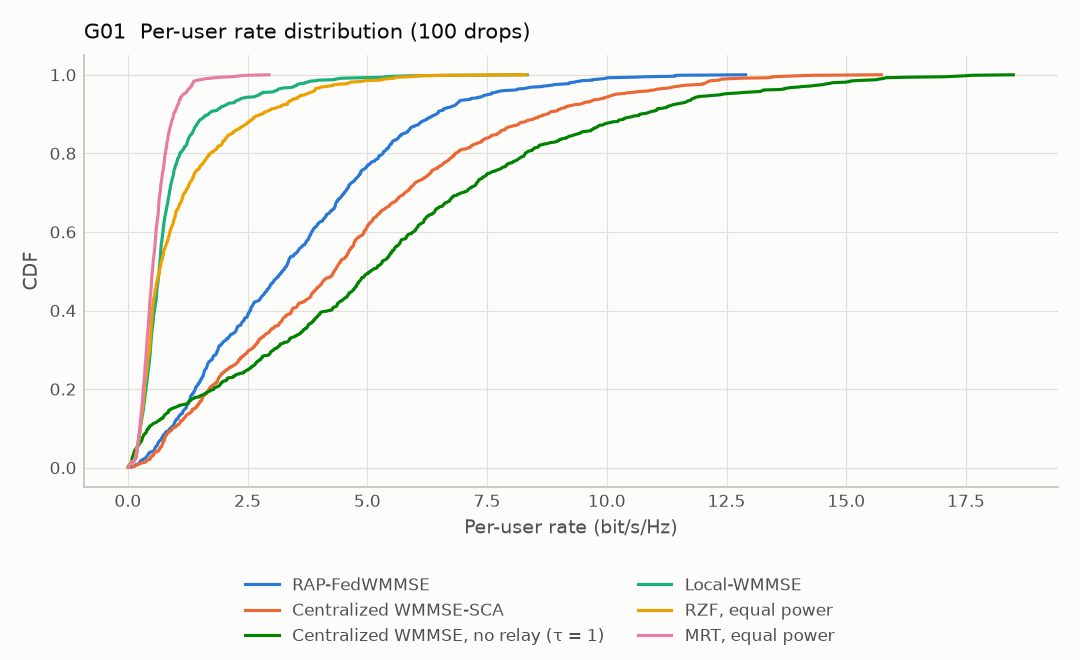
\includegraphics[width=\columnwidth]{G01_rate_cdf.png}
\caption{Per-user rate CDF on the default network. Relays trade median rate
for the tail: the no-relay benchmark wins the median and loses the 5th
percentile by $3\times$.}
\label{fig:g01}
\end{figure}

\begin{figure}[t]
\centering
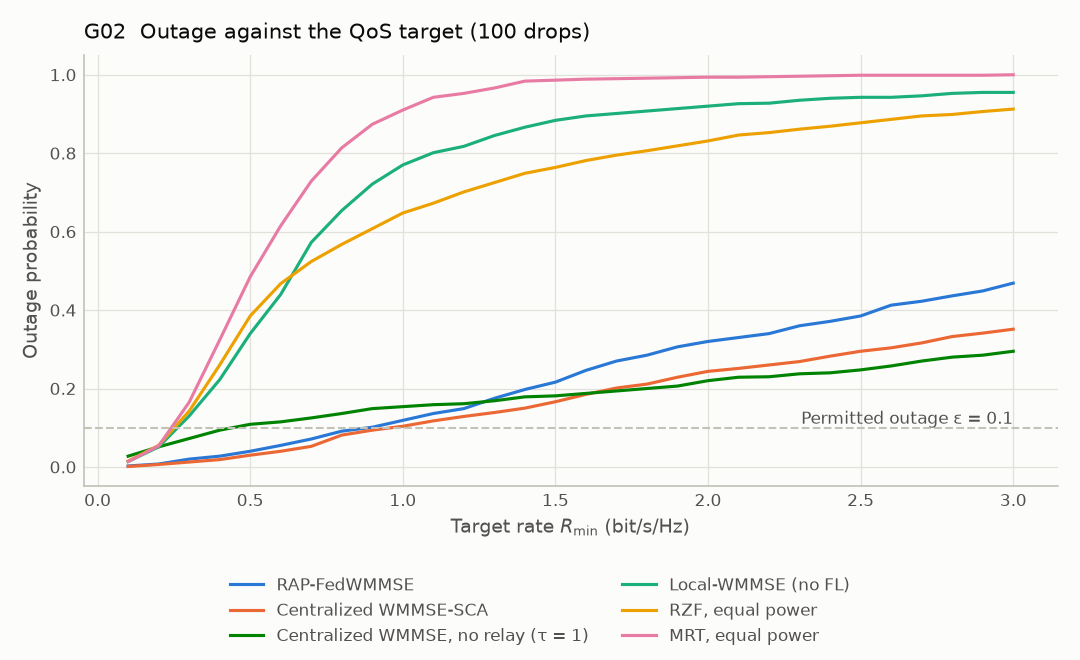
\includegraphics[width=\columnwidth]{G02_outage.png}
\caption{Outage probability against the QoS target $R^{\min}$.}
\label{fig:g02}
\end{figure}

\subsection{Power, load and blockage (Figs.~\ref{fig:g03}--\ref{fig:g05})}
Across transmit powers from 10 to 30\,dBm (Fig.~\ref{fig:g03}), the ordering
is stable. The 5th-percentile panel shows the relay methods turning extra
power into tail rate much faster than the no-relay benchmark. Against the
number of UEs (Fig.~\ref{fig:g04}), every method peaks at $K=8$ and declines
as load grows. RAP-FedWMMSE declines faster than the centralized method
($7.88\to4.80$ against $9.88\to8.02$ from $K=8$ to $12$), which we attribute
to a fixed number of layers facing a harder interference problem.

The blockage sweep (Fig.~\ref{fig:g05}) shows what relays are for. Without
blockage, the no-relay benchmark is \emph{better} by 1.86, because it spends
the whole frame on direct links. At 75\% blocked UEs, the relay-assisted
centralized method wins by $0.97\pm0.43$.

\begin{figure}[t]
\centering
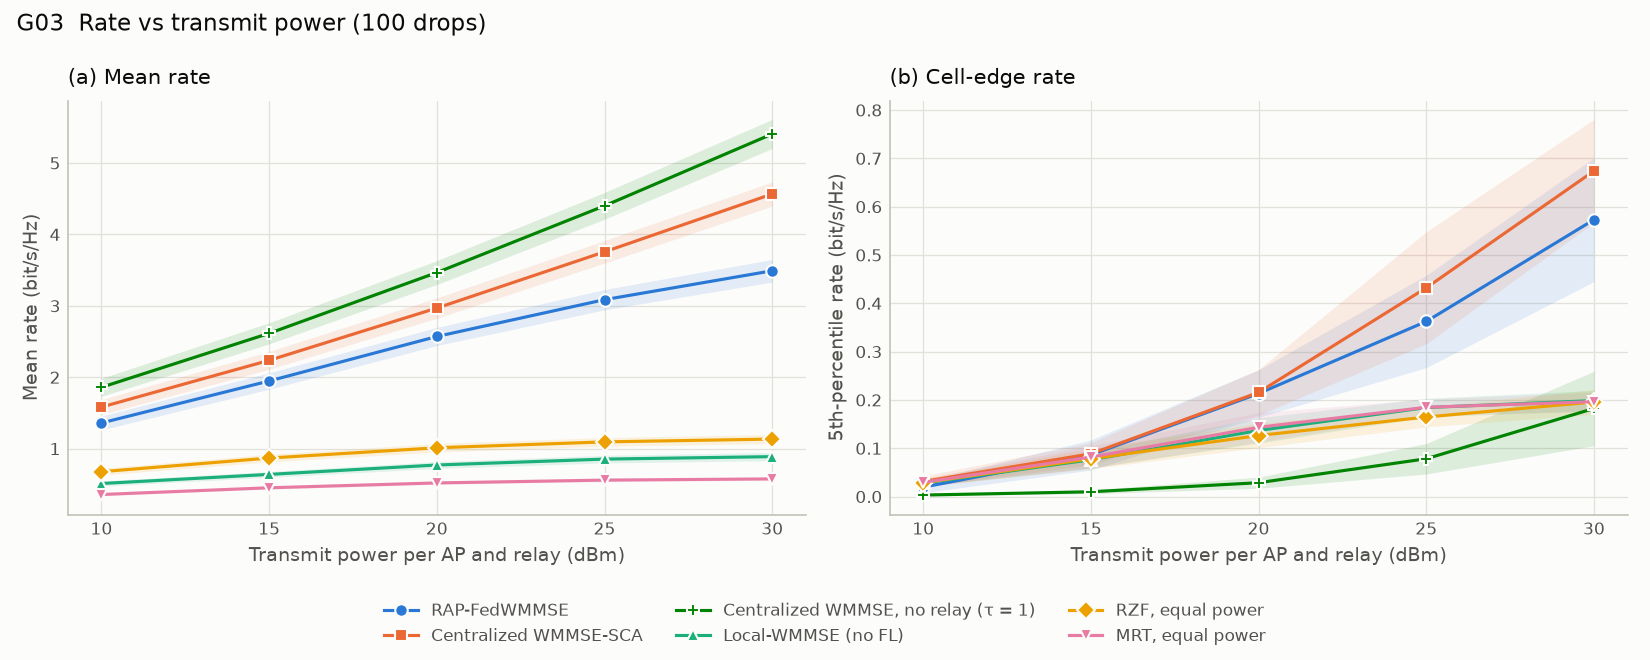
\includegraphics[width=\columnwidth]{G03_rate_vs_power.png}
\caption{(a) Mean and (b) 5th-percentile rate against per-node transmit
power.}
\label{fig:g03}
\end{figure}

\begin{figure}[t]
\centering
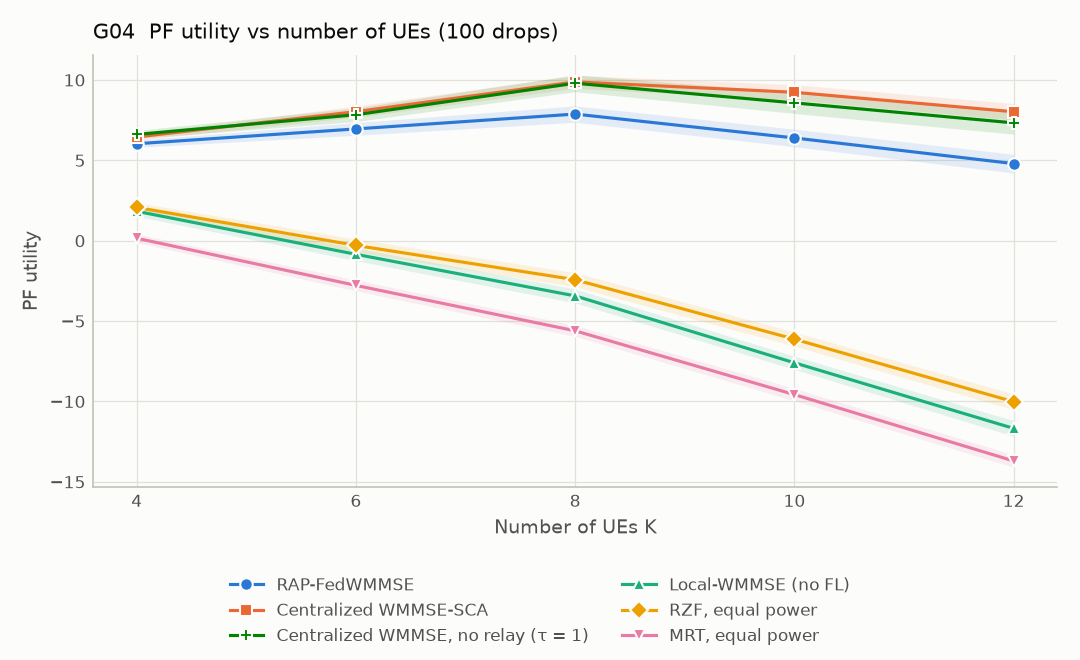
\includegraphics[width=\columnwidth]{G04_pf_vs_ues.png}
\caption{PF utility against the number of UEs (a separate model is trained
for each $K$).}
\label{fig:g04}
\end{figure}

\begin{figure}[t]
\centering
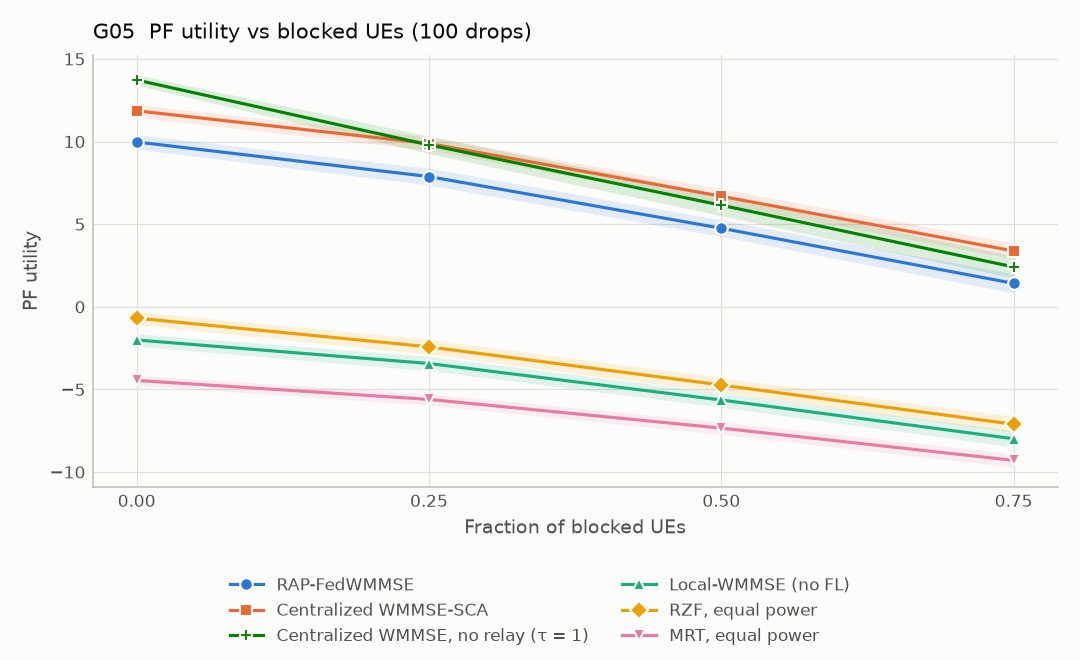
\includegraphics[width=\columnwidth]{G05_pf_vs_blocked.png}
\caption{PF utility against the fraction of blocked UEs. The relay gain is a
blockage gain.}
\label{fig:g05}
\end{figure}

\subsection{Relays, cooperation and the phase split (Figs.~\ref{fig:g06},
\ref{fig:g07})}\label{sec:coop}
More relays help, with diminishing returns (Fig.~\ref{fig:g06}): centralized
utility grows from 9.32 at $R=1$ to 9.97 at $R=4$. Cooperative forwarding
($L_{\max}=2$, dashed) slightly \emph{lowers} utility, by 0.19 for the
centralized method and 0.81 for RAP-FedWMMSE at $R=2$. This is a direct
consequence of assumption~(iii): every assisting relay must decode, so the
weaker relay's hop becomes the bottleneck. It did not support our hypothesis
that cooperation would help at these sizes.

The fixed-$\tau$ sweep (Fig.~\ref{fig:g07}) rises monotonically over
$[0.2,0.8]$ for every relay-assisted method: Phase~I carries most of the
rate. For RAP-FedWMMSE, fixing $\tau=0.5$ instead of $0.8$ costs about 3
utility, consistent with the $+3.12$ of the slow timescale in
Table~\ref{tab:decomp}.

\begin{figure}[t]
\centering
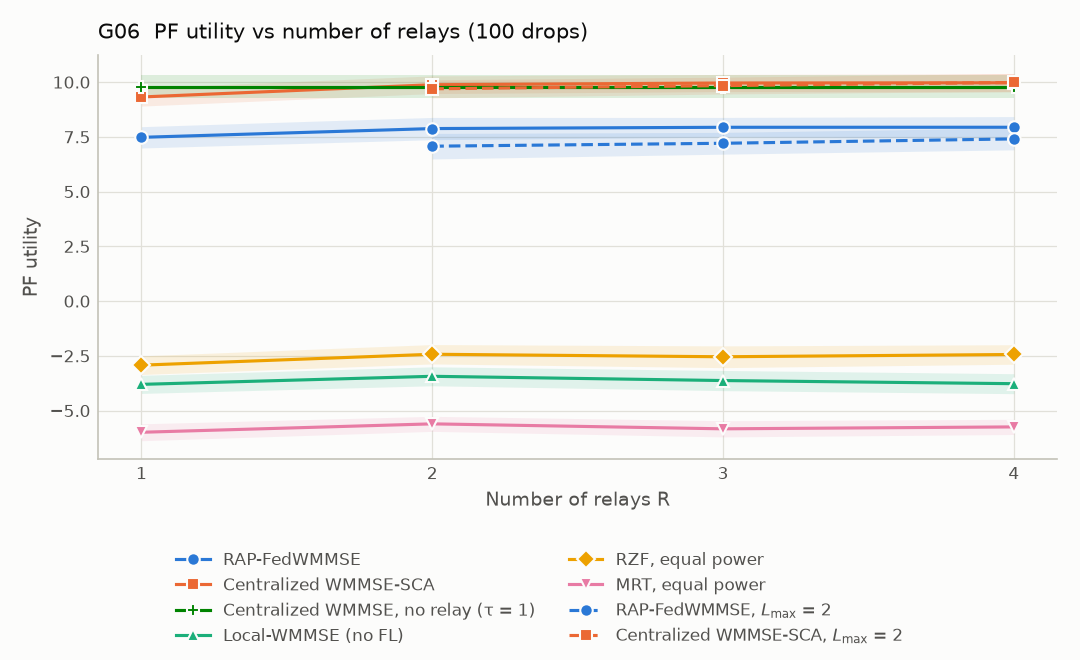
\includegraphics[width=\columnwidth]{G06_pf_vs_relays.png}
\caption{PF utility against the number of relays, with $L_{\max}=1$ (solid)
and cooperative forwarding $L_{\max}=2$ (dashed).}
\label{fig:g06}
\end{figure}

\begin{figure}[t]
\centering
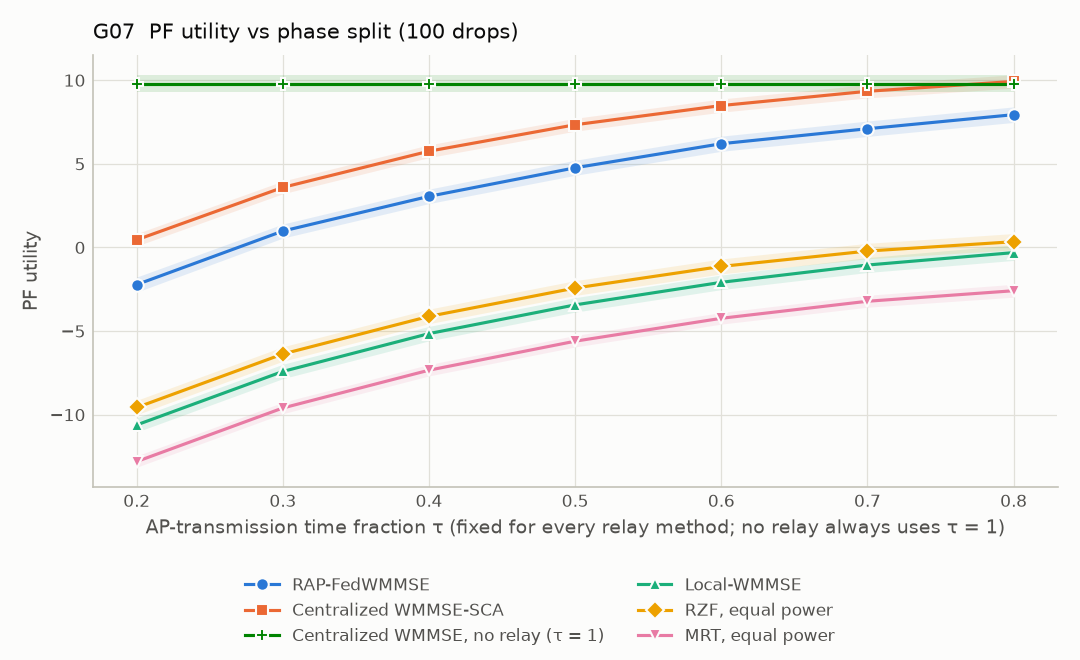
\includegraphics[width=\columnwidth]{G07_pf_vs_tau.png}
\caption{PF utility against a fixed phase split $\tau$ (association fixed,
same drops for every method).}
\label{fig:g07}
\end{figure}

\subsection{Robustness to stale CSI (Fig.~\ref{fig:g08})}
Under channel aging $\mathbf{H} = \rho\hat{\mathbf{H}} +
\sqrt{1-\rho^2}\,\mathbf{E}$, RAP-FedWMMSE overtakes the centralized
relay-assisted benchmark for $\rho\le0.9$: by $+1.01\pm0.40$ at $\rho=0.8$,
$+0.78$ at 0.85 and $+0.62$ at 0.9 (paired). The comparison is asymmetric by
design. RAP-FedWMMSE is retrained at every $\rho$ with the matching error
model of Section~\ref{sec:robust}, while the centralized benchmark is
certainty-equivalent. The result therefore shows the value of robust
training, not that the learned layers beat a robust centralized optimizer,
which we did not implement.

The no-relay benchmark stays above both in PF utility. Against it,
RAP-FedWMMSE is lower by $0.29\pm0.54$, $0.48\pm0.49$ and $0.49\pm0.44$ at
$\rho=0.8$, 0.85 and 0.9; only the last is significant. RAP-FedWMMSE keeps
the better tail at every $\rho$: its 5th-percentile rate is 0.15 against 0.08
at $\rho=0.8$, and 0.25 against 0.14 at 0.9, and its outage is lower (23.0\%
against 24.1\% at 0.8, and 11.4\% against 15.1\% at 0.9).

\begin{figure}[t]
\centering
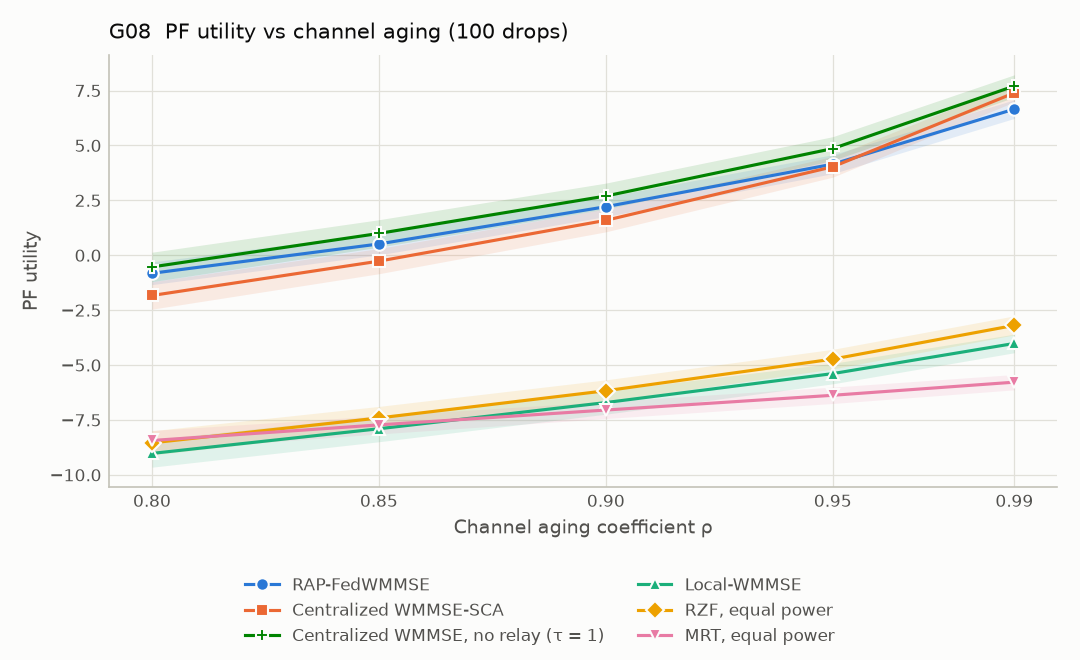
\includegraphics[width=\columnwidth]{G08_pf_vs_aging.png}
\caption{PF utility against the aging coefficient $\rho$. RAP-FedWMMSE is
retrained at each $\rho$ with the matching error model; the centralized
benchmarks are certainty-equivalent.}
\label{fig:g08}
\end{figure}

\subsection{What the learning adds (Figs.~\ref{fig:g09}, \ref{fig:g12})}
With $\tau$ and association held fixed (Fig.~\ref{fig:g09}), the trained
layers beat the identical untrained layers at every depth: by $+1.37$ at
$L=1$, $+0.89\pm0.16$ at $L=6$ and $+0.64$ at $L=10$. Six trained layers
roughly match ten untrained ones (4.76 against 4.74). Learned step sizes
matter most when there are few iterations, but their effect is modest. The
larger default-configuration margin of $+4.0$ over the untrained ablation is
mostly the slow timescale (Table~\ref{tab:decomp}).

Fig.~\ref{fig:g12} shows the federated training. Validation utility starts
near 6.8 after the first epoch, because $\tau$ has already been adapted
(to 0.75--0.8 on every deployment) and the validation runs the warm-up. It
plateaus near 7.5--7.6 within about 20 epochs. Validation uses 4 separate
drops per deployment, so its level differs from the 100-drop evaluation mean
of 7.88 within sampling variation. The personalized scheme reaches the same
plateau as FedAvg with 45\% less communication (11\,MB against 20\,MB).

\begin{figure}[t]
\centering
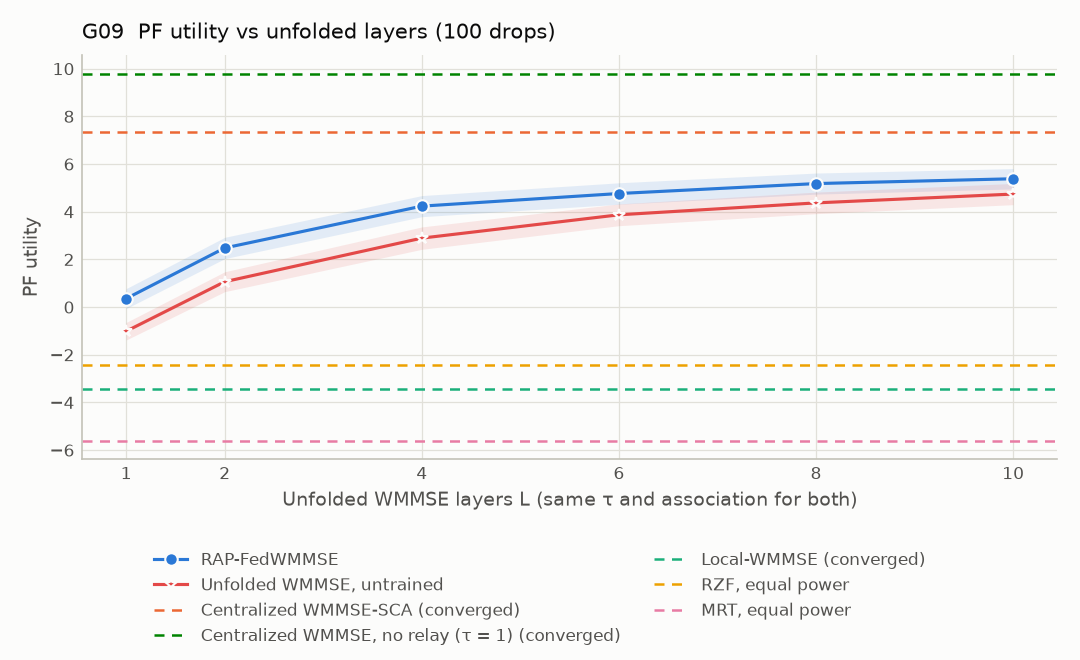
\includegraphics[width=\columnwidth]{G09_pf_vs_layers.png}
\caption{PF utility against the number of unfolded layers $L$, trained
against untrained, with every other method as a reference line (all at
$\tau=0.5$, fixed association).}
\label{fig:g09}
\end{figure}

\subsection{Distance from the global optimum (Fig.~\ref{fig:g10})}
On the small network, SCIP certified the global bound to a 1\% gap on 94 of
100 drops. The other 6 hit the time limit, where the bound remains valid.
The mean gaps to the certified bound are:
\begin{itemize}
  \item exact incumbent 0.04;
  \item centralized WMMSE 0.35;
  \item untrained unfolded layers 0.80;
  \item RAP-FedWMMSE 1.12;
  \item Local-WMMSE 1.64;
  \item MRT 1.77.
\end{itemize}
No method exceeded the bound in 600 records.

The centralized method's local optima are nearly global here, which supports
its use as a benchmark. \emph{Trained} RAP-FedWMMSE, however, falls below its
own untrained layers on this single-antenna network and nearly starves one
UE on 14 of 100 drops. This model was trained from scratch on the small
network, with the hyperparameters chosen for the default network. With
$N_A=N_R=1$ the beams have no spatial freedom, so each layer reduces to power
control. Our hypothesis, which we have not verified, is that the learned
initial power shares and step sizes can then drive one stream towards zero.
The effect does not occur on the default network, and we report it as a
limitation rather than tune it away.

\begin{figure}[t]
\centering
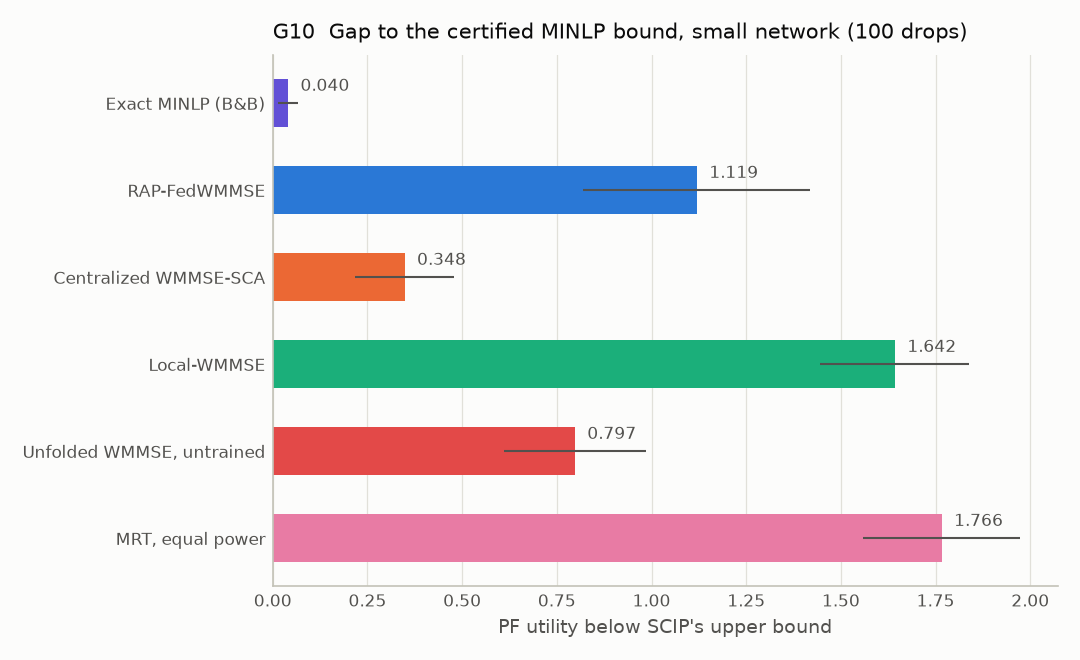
\includegraphics[width=\columnwidth]{G10_optimality_gap.png}
\caption{Gap to the certified MINLP upper bound on the small network (2 APs,
1 relay, 2 UEs; every method at $\tau=0.5$).}
\label{fig:g10}
\end{figure}

\subsection{Runtime (Fig.~\ref{fig:g11})}\label{sec:runtime}
In the runtime sweep, RAP-FedWMMSE's inference time, including its warm-up,
stays at 0.33--0.38\,s from $K=4$ to 12, while centralized WMMSE grows from
about 2\,s to about 48\,s. Most of RAP-FedWMMSE's time is the warm-up: in the
main run, the untrained layers, which skip it, took 0.09\,s per drop. Three
caveats limit this comparison:
\begin{itemize}
  \item \textbf{Solvers differ.} The centralized benchmark calls a
    general-purpose conic solver through CVXPY at every iteration, which
    keeps the DF $\min$ and log utility exact. The unfolded layers are
    closed-form tensor operations. Much of the gap is this implementation
    difference rather than an algorithmic one; even the no-relay centralized
    method takes about 4.7\,s.
  \item \textbf{One process, no communication delay.} Times are wall-clock in
    one process, with all nodes computed together as batched tensors. They
    exclude the $L$ sequential $\zf$ exchanges a physical network would need
    per block.
  \item \textbf{Timings are noisy.} They were measured with 11 parallel
    workers on 12 cores and vary with load. In the main run, the three
    RAP-FedWMMSE variants, whose inference is identical, took 0.32\,s to
    1.3\,s per drop, and the centralized method 38\,s.
\end{itemize}
We therefore claim only an order-of-magnitude advantage in computation.

\begin{figure}[t]
\centering
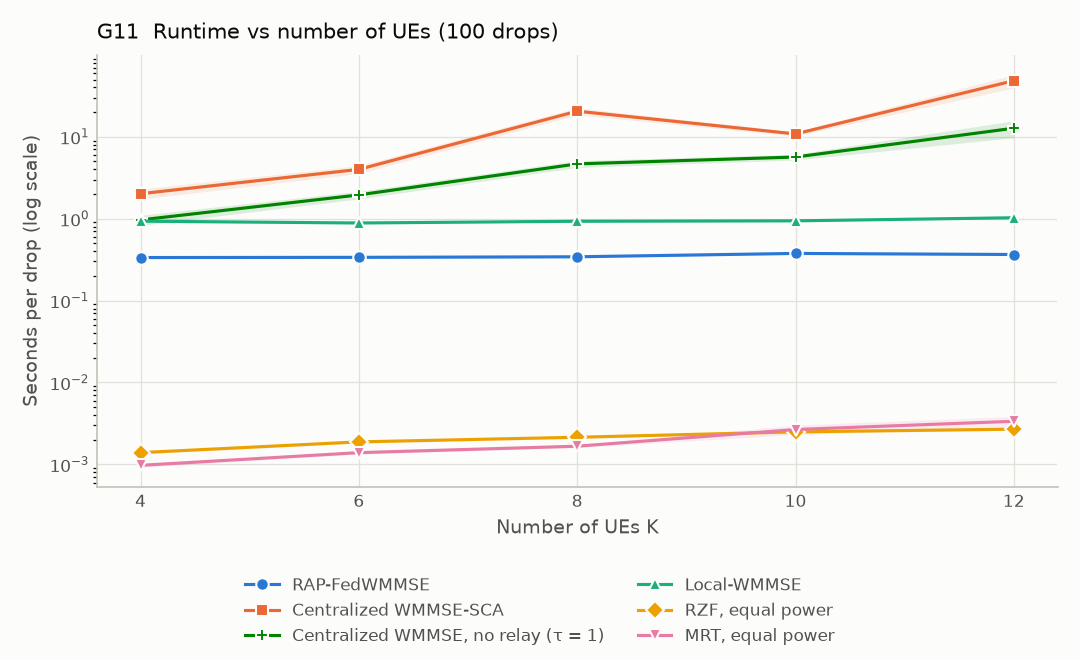
\includegraphics[width=\columnwidth]{G11_runtime_vs_ues.png}
\caption{Single-process inference time per drop against the number of UEs
(log scale); per-layer exchange latency is not included.}
\label{fig:g11}
\end{figure}

\begin{figure*}[t]
\centering
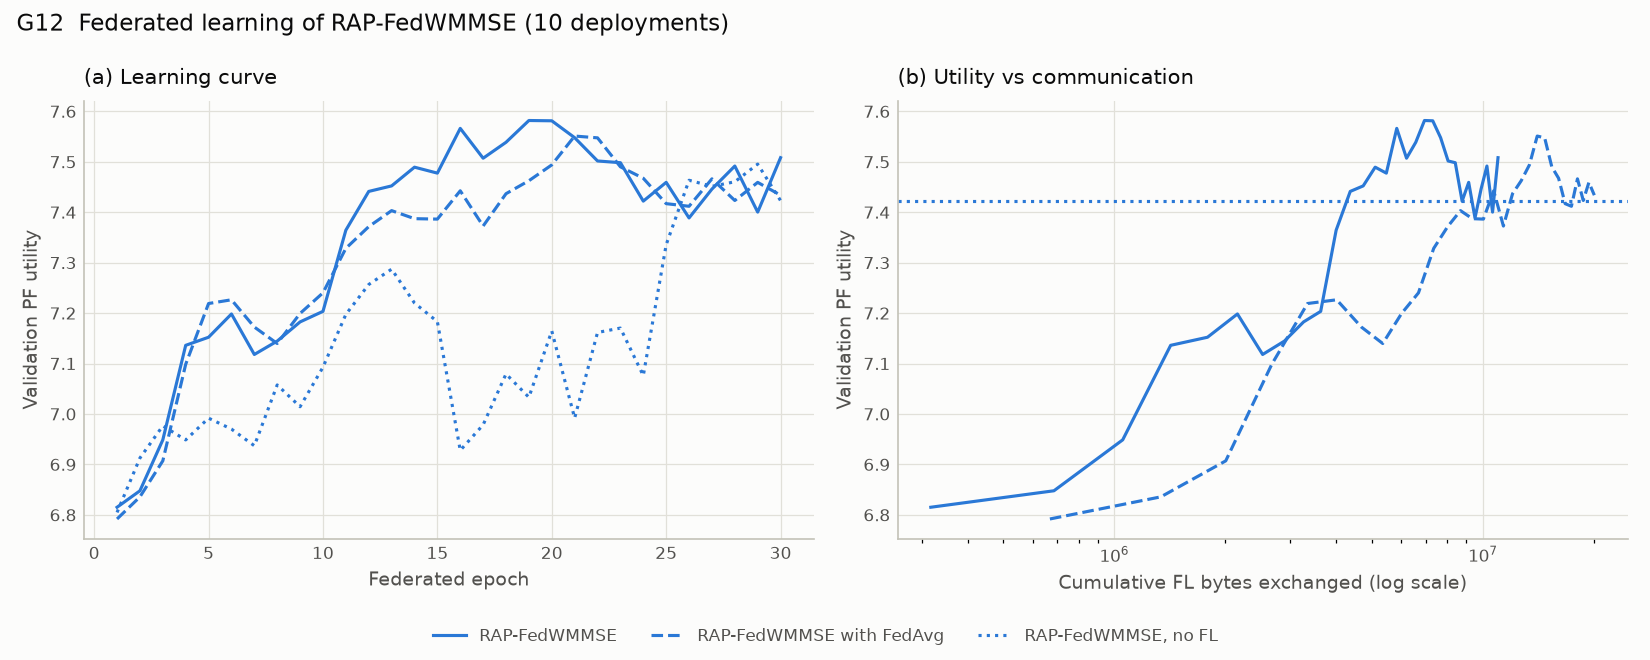
\includegraphics[width=0.85\textwidth]{G12_fl_learning.png}
\caption{Federated learning dynamics: validation PF utility against (a)
federated epoch and (b) cumulative communicated bytes, for personalized
aggregation, FedAvg and no federation.}
\label{fig:g12}
\end{figure*}

\subsection{Energy (Fig.~\ref{fig:g13})}
Sweeping the energy price $\lambda_E$ traces each method's utility--power
frontier. At $\lambda_E=0.1$, RAP-FedWMMSE cuts $P_{\mathrm{tot}}$
\eqref{eq:ptot} from 23.9 to 18.7\,W (22\%) for a utility loss of 0.14. At
$\lambda_E=0.5$ it runs at 8.6\,W. The centralized frontiers have a similar
shape. The heuristics always transmit at full power and appear as single
points.

\begin{figure}[t]
\centering
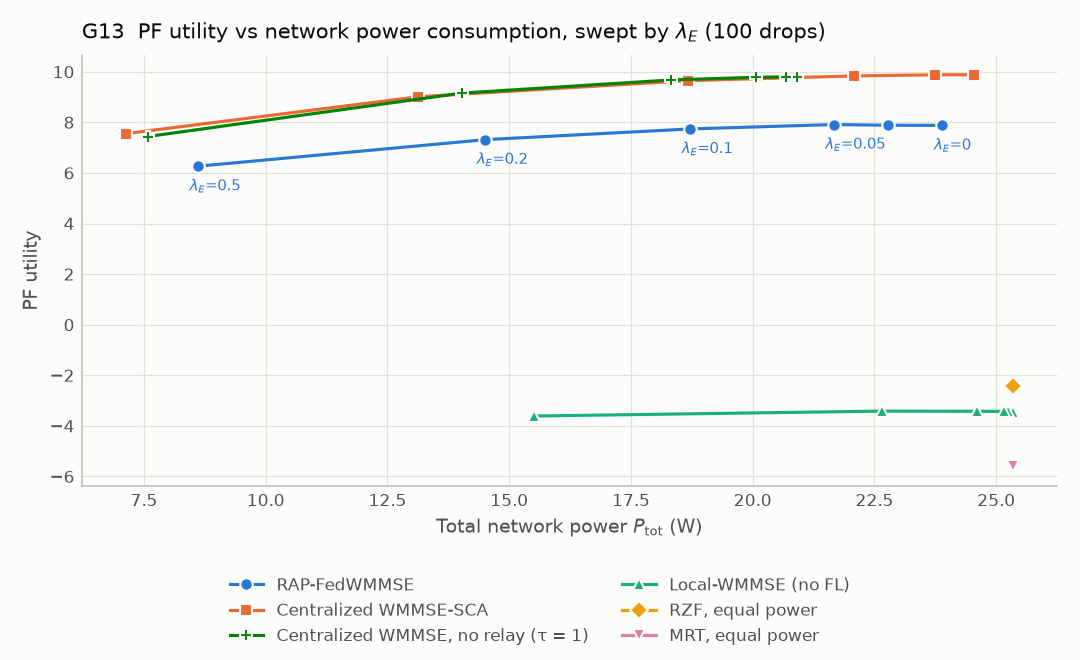
\includegraphics[width=\columnwidth]{G13_energy_tradeoff.png}
\caption{PF utility against network power consumption, swept by the energy
price $\lambda_E$.}
\label{fig:g13}
\end{figure}

\subsection{Federation under the fronthaul constraint (Fig.~\ref{fig:g14})
and a negative result}
Fig.~\ref{fig:g14} enforces \eqref{eq:fronthaul} on the FL traffic while
sweeping the AP fronthaul capacity. At 100\,Mbit/s, an average of 7.1 of 8
APs are overloaded by user data alone, and FL participation falls to 2.8 of
10 nodes per epoch. FedAvg reaches full participation only at 1\,Gbit/s,
while the personalized scheme is capped at five uploads per epoch by
$B_{\mathrm{FL}}$. As stated in Section~\ref{sec:problem}, the overloaded APs' user rates are
not reduced, so Fig.~\ref{fig:g14}(a) shows the effect of the constraint on
learning only.

Utility is flat across the sweep, which exposes the negative result:
\textbf{in this setting, federated aggregation does not measurably improve
utility over training without it}. Personalized, FedAvg and no-FL agree
within noise ($-0.06\pm0.19$ paired difference between personalized and
no-FL). We see two reasons. First, every node trains self-supervised on
unlimited fresh realizations of its own deployment, so local training already
saturates; each node effectively owns a perfect simulator. Second, as stated
in Section~\ref{sec:train}, training backpropagates the global objective through all
nodes, so even the no-FL nodes learn from network-wide gradients rather than
in isolation. Both assumptions favor the no-FL baseline.

The demonstrated value of Steps~12--15 is therefore communication efficiency
--- 45\% less traffic than FedAvg for the same utility, and graceful behavior
under fronthaul scarcity --- not a utility gain. Showing a utility gain would
need a regime with limited local data, heterogeneous nodes and truly local
gradients. We leave this as future work.

\begin{figure*}[t]
\centering
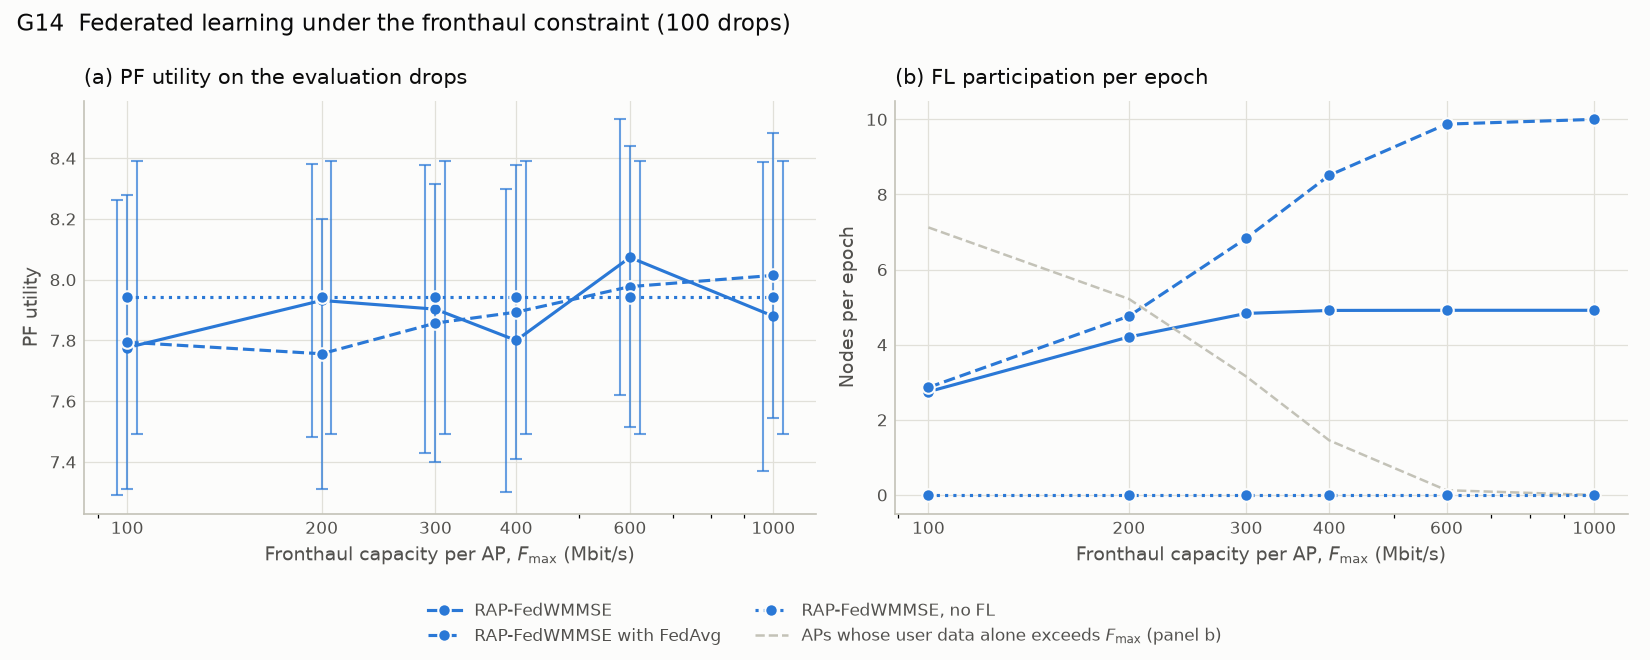
\includegraphics[width=0.85\textwidth]{G14_fronthaul.png}
\caption{Federation under the fronthaul constraint \eqref{eq:fronthaul}: (a)
PF utility and (b) FL participation and overloaded APs against per-AP
fronthaul capacity.}
\label{fig:g14}
\end{figure*}

\subsection{Limitations}
\begin{enumerate}
  \item[(i)] Federation shows no utility gain in our regime, in which
    training has unlimited data and network-wide gradients.
  \item[(ii)] The learned layer parameters add $+0.9$ PF at $L=6$; most of
    the gain comes from coordination and slow-timescale adaptation.
  \item[(iii)] On the small single-antenna network, the trained model
    underperforms its untrained layers and nearly starves a UE on 14\% of
    drops.
  \item[(iv)] Cooperative forwarding ($L_{\max}=2$) slightly lowers utility.
  \item[(v)] The fast exchange costs more than raw CSI upload at 2 antennas,
    and its latency and the training-time backward exchange are not
    modeled.
  \item[(vi)] The fronthaul constraint gates FL only. $P_{\mathrm{tot}}$ is
    the power drawn while transmitting, not its time average.
  \item[(vii)] Training carries $\zs$ across UE drops.
  \item[(viii)] The aging comparison uses a certainty-equivalent centralized
    benchmark.
  \item[(ix)] CSI acquisition is not modeled; each drop is one coherence
    block; antenna counts are small.
  \item[(x)] Runtimes are indicative only, to an order of magnitude.
\end{enumerate}

\section{Conclusion}
We implemented RAP-FedWMMSE end to end and evaluated it against centralized,
local, heuristic and certified-exact benchmarks across 14 experiments. Its
parts are:
\begin{itemize}
  \item capacitated relay association and an adaptive phase split;
  \item role-aware models over a personalized backbone;
  \item unfolded WMMSE layers that reduce exactly to the classical update;
  \item primal--dual QoS/DF correction;
  \item robust self-supervised training without any dataset;
  \item event-triggered, budgeted, compressed, personalized federation under
    fronthaul limits.
\end{itemize}
The method delivers near-centralized tail performance for blocked users at
an order of magnitude less computation, and $+11.3$ PF utility over
uncoordinated local optimization. It also overtakes certainty-equivalent
centralized optimization under stale CSI, and gives a clean energy--utility
trade-off.

The paired decomposition shows where this comes from: mostly the per-layer
coordination ($+7.3$) and the slow-timescale Steps~1--2 ($+3.1$), and only
modestly the learned parameters ($+0.9$). The certified bounds and paired
statistics also show what the method does not deliver at this scale:
\begin{itemize}
  \item a utility gain from federation;
  \item gains from cooperative forwarding;
  \item reliability on degenerate single-antenna networks.
\end{itemize}
Future work is to test federation where its premise holds --- limited data,
heterogeneous nodes and truly local gradients --- and to model the latency of
the coordination exchange.

\section*{Reproducibility}
All code, configuration, seeds and the exact commands that regenerate every
figure and table accompany this submission. All channels are synthetic and
generated by the included simulator; no external dataset is used. The command
\texttt{run\_experiments.py --drops 100 --deployments 10} reproduces the
reported results from seed 42.

\begin{thebibliography}{00}
\bibitem{ngo2017cellfree} H.~Q. Ngo, A.~Ashikhmin, H.~Yang, E.~G. Larsson,
and T.~L. Marzetta, ``Cell-free massive MIMO versus small cells,''
\emph{IEEE Trans. Wireless Commun.}, vol.~16, no.~3, pp. 1834--1850, Mar.
2017.
\bibitem{interdonato2019ubiquitous} G.~Interdonato, E.~Bj\"ornson, H.~Q.
Ngo, P.~Frenger, and E.~G. Larsson, ``Ubiquitous cell-free massive MIMO
communications,'' \emph{EURASIP J. Wireless Commun. Netw.}, vol. 2019,
no.~1, p. 197, 2019.
\bibitem{cover1979relay} T.~Cover and A.~El~Gamal, ``Capacity theorems for
the relay channel,'' \emph{IEEE Trans. Inf. Theory}, vol.~25, no.~5, pp.
572--584, Sep. 1979.
\bibitem{laneman2004cooperative} J.~N. Laneman, D.~N.~C. Tse, and G.~W.
Wornell, ``Cooperative diversity in wireless networks: Efficient protocols
and outage behavior,'' \emph{IEEE Trans. Inf. Theory}, vol.~50, no.~12, pp.
3062--3080, Dec. 2004.
\bibitem{shi2011wmmse} Q.~Shi, M.~Razaviyayn, Z.-Q. Luo, and C.~He, ``An
iteratively weighted MMSE approach to distributed sum-utility maximization
for a MIMO interfering broadcast channel,'' \emph{IEEE Trans. Signal
Process.}, vol.~59, no.~9, pp. 4331--4340, Sep. 2011.
\bibitem{christensen2008wmmse} S.~S. Christensen, R.~Agarwal, E.~de
Carvalho, and J.~M. Cioffi, ``Weighted sum-rate maximization using weighted
MMSE for MIMO-BC beamforming design,'' \emph{IEEE Trans. Wireless Commun.},
vol.~7, no.~12, pp. 4792--4799, Dec. 2008.
\bibitem{monga2021unrolling} V.~Monga, Y.~Li, and Y.~C. Eldar, ``Algorithm
unrolling: Interpretable, efficient deep learning for signal and image
processing,'' \emph{IEEE Signal Process. Mag.}, vol.~38, no.~2, pp. 18--44,
Mar. 2021.
\bibitem{chowdhury2021unfolding} A.~Chowdhury, G.~Verma, C.~Rao, A.~Swami,
and S.~Segarra, ``Unfolding WMMSE using graph neural networks for efficient
power allocation,'' \emph{IEEE Trans. Wireless Commun.}, vol.~20, no.~9,
pp. 6004--6017, Sep. 2021.
\bibitem{hu2021iaidnn} Q.~Hu, Y.~Cai, Q.~Shi, K.~Xu, G.~Yu, and Z.~Ding,
``Iterative algorithm induced deep-unfolding neural networks: Precoding
design for multiuser MIMO systems,'' \emph{IEEE Trans. Wireless Commun.},
vol.~20, no.~2, pp. 1394--1410, Feb. 2021.
\bibitem{pellaco2022inversefree} L.~Pellaco, M.~Bengtsson, and J.~Jald\'en,
``Matrix-inverse-free deep unfolding of the weighted MMSE beamforming
algorithm,'' \emph{IEEE Open J. Commun. Soc.}, vol.~3, pp. 65--81, 2022.
\bibitem{schynol2023gcnwmmse} L.~Schynol and M.~Pesavento, ``Coordinated
sum-rate maximization in multicell MU-MIMO with deep unrolling,''
\emph{IEEE J. Sel. Areas Commun.}, vol.~41, no.~4, pp. 1120--1134, Apr.
2023.
\bibitem{miretti2022team} L.~Miretti, E.~Bj\"ornson, and D.~Gesbert, ``Team
MMSE precoding with applications to cell-free massive MIMO,'' \emph{IEEE
Trans. Wireless Commun.}, vol.~21, no.~8, pp. 6242--6255, Aug. 2022.
\bibitem{nguyen2023hrris} N.~T. Nguyen, V.-D. Nguyen, H.~V. Nguyen, H.~Q.
Ngo, S.~Chatzinotas, and M.~Juntti, ``Spectral efficiency analysis of hybrid
relay-reflecting intelligent surface-assisted cell-free massive MIMO
systems,'' \emph{IEEE Trans. Wireless Commun.}, vol.~22, no.~5, pp.
3397--3416, May 2023.
\bibitem{vu2023dfrelay} T.~T. Vu, H.~Q. Ngo, M.~N. Dao, and E.~G. Larsson,
``Multipair DF relaying with network-assisted full-duplex cell-free massive
MIMO,'' in \emph{Proc. EUSIPCO}, 2023, pp. 1474--1478.
\bibitem{mcmahan2017fedavg} B.~McMahan, E.~Moore, D.~Ramage, S.~Hampson,
and B.~A. y~Arcas, ``Communication-efficient learning of deep networks from
decentralized data,'' in \emph{Proc. AISTATS}, 2017, pp. 1273--1282.
\bibitem{tan2022personalized} A.~Z. Tan, H.~Yu, L.~Cui, and Q.~Yang,
``Towards personalized federated learning,'' \emph{IEEE Trans. Neural Netw.
Learn. Syst.}, vol.~34, no.~12, pp. 9587--9603, 2023.
\bibitem{aji2017sparse} A.~F. Aji and K.~Heafield, ``Sparse communication
for distributed gradient descent,'' in \emph{Proc. EMNLP}, 2017, pp.
440--445.
\bibitem{wang2023flprecoding} D.~Wang, M.~Tao, X.~Zeng, and J.~Liang,
``Federated learning for precoding design in cell-free massive MIMO
systems,'' \emph{IEEE Open J. Commun. Soc.}, vol.~4, pp. 1567--1582, 2023.
\bibitem{bestuzheva2021scip} K.~Bestuzheva \emph{et~al.}, ``The SCIP
optimization suite 8.0,'' Zuse Institute Berlin, Tech. Rep., 2021.
\end{thebibliography}

\end{document}
